\PassOptionsToPackage{obeyspaces,spaces}{url}
\documentclass[11pt,a4paper]{article}

% ------------------------------------------------------------------
% Layout and fonts
% ------------------------------------------------------------------
\usepackage[T1]{fontenc}
\usepackage[utf8]{inputenc}
\usepackage[scaled=0.92]{helvet}
\usepackage{mathpazo}
\usepackage{inconsolata}
\usepackage[a4paper,margin=24mm,headheight=14pt]{geometry}
\usepackage{microtype}
\usepackage{amsmath,amssymb}
\usepackage{xcolor}
\usepackage{graphicx}
\usepackage{booktabs,tabularx,longtable,array}
\usepackage{enumitem}
\usepackage{fancyhdr}
\usepackage{titlesec}
\usepackage{caption}
\usepackage{listings}
\usepackage{tikz}
\usetikzlibrary{arrows.meta,positioning}
\usepackage[most]{tcolorbox}
\usepackage[hidelinks]{hyperref}
\usepackage{url}
\usepackage{needspace}
\usepackage{placeins}
\usepackage{tocloft}
\setlength{\cftbeforesecskip}{3pt}
\renewcommand{\cftsecfont}{\sffamily\small\bfseries}
\renewcommand{\cftsecpagefont}{\sffamily\small\bfseries}
\renewcommand{\cftsubsecfont}{\small}
\renewcommand{\cftsubsecpagefont}{\small}
\setlength{\cftbeforesubsecskip}{0pt}
\renewcommand{\cfttoctitlefont}{\sffamily\Large\bfseries\color{accent}}

\definecolor{ink}{HTML}{1B1B1A}
\definecolor{muted}{HTML}{5D5C58}
\definecolor{rule}{HTML}{D8D7D2}
\definecolor{accent}{HTML}{1C5CAB}
\definecolor{okc}{HTML}{0B7A0B}
\definecolor{specc}{HTML}{1C5CAB}
\definecolor{partc}{HTML}{9A6200}
\definecolor{noc}{HTML}{6F6E6A}
\definecolor{warnc}{HTML}{B3261E}
\definecolor{boxbg}{HTML}{F6F6F3}
\definecolor{longc}{HTML}{2A78D6}
\definecolor{shortc}{HTML}{EB6834}

\color{ink}
\hypersetup{colorlinks=true,linkcolor=accent,urlcolor=accent,citecolor=accent}
\setlength{\parindent}{0pt}
\setlength{\parskip}{6pt plus 1pt}
\setlist{itemsep=2pt,topsep=3pt,parsep=0pt}
\setlist[enumerate,1]{label=\textbf{\arabic*.},leftmargin=*,widest=9}
\captionsetup{font=small,labelfont=bf,labelsep=period,justification=raggedright,singlelinecheck=false}
\renewcommand{\arraystretch}{1.15}
\emergencystretch=2em

\titleformat{\section}{\sffamily\Large\bfseries\color{accent}}{\thesection}{0.6em}{}
\titleformat{\subsection}{\sffamily\large\bfseries}{\thesubsection}{0.6em}{}
\titleformat{\subsubsection}{\sffamily\normalsize\bfseries}{}{0em}{}
\titlespacing*{\section}{0pt}{16pt}{6pt}
\titlespacing*{\subsection}{0pt}{13pt}{4pt}
\titlespacing*{\subsubsection}{0pt}{9pt}{2pt}

\pagestyle{fancy}
\fancyhf{}
\fancyhead[L]{\sffamily\footnotesize\color{muted}Positioning and Pain Monitors: replication specification}
\fancyhead[R]{\sffamily\footnotesize\color{muted}Private}
\fancyfoot[C]{\sffamily\footnotesize\color{muted}\thepage}
\renewcommand{\headrulewidth}{0.3pt}

\lstdefinestyle{code}{basicstyle=\ttfamily\footnotesize,columns=fullflexible,keepspaces=true,breaklines=true,
  breakatwhitespace=false,showstringspaces=false,frame=none,xleftmargin=0pt,aboveskip=4pt,belowskip=4pt,
  keywordstyle=\color{accent},commentstyle=\color{muted},stringstyle=\color{ink},literate={−}{{-}}1 {×}{{x}}1}
\lstdefinestyle{shell}{style=code,language=bash,backgroundcolor=\color{boxbg},framesep=4pt,frame=single,rulecolor=\color{rule}}
\lstdefinestyle{py}{style=code,language=Python,basicstyle=\ttfamily\scriptsize}
\lstset{style=code}

% ------------------------------------------------------------------
% Own commands
% ------------------------------------------------------------------
\def\UrlBreaks{\do\/\do\-\do\_\do\.\do\=}
\Urlmuskip=0mu
\urlstyle{tt}
\newcommand{\code}[1]{\nolinkurl{#1}}
\newcommand{\chip}[2]{\textcolor{#1}{\sffamily\footnotesize\bfseries[#2]}}
\newcommand{\Verified}{\chip{okc}{Verified}}
\newcommand{\Specified}{\chip{specc}{Specified}}
\newcommand{\Partial}{\chip{partc}{Partial}}
\newcommand{\NotRep}{\chip{noc}{Not replicable}}
\newcommand{\method}[3]{\FloatBarrier\subsection[#1 #2]{#1 \quad #2}\vspace{-2pt}{#3}\par}
\newcommand{\sublabel}[1]{\par\vspace{3pt}\needspace{3\baselineskip}{\sffamily\small\bfseries #1}\par\nopagebreak[4]\vspace{1pt}}
\newcolumntype{L}{>{\raggedright\arraybackslash}X}
\newcolumntype{P}[1]{>{\raggedright\arraybackslash}p{#1}}

\newtcolorbox{decision}[1][]{enhanced,breakable,colback=boxbg,colframe=specc,boxrule=0pt,leftrule=2.5pt,arc=0pt,
  left=7pt,right=6pt,top=3pt,bottom=3pt,fontupper=\small,before skip=6pt,after skip=6pt,
  title={Decisions. The source is silent, so this specification chooses.},coltitle=specc,colbacktitle=boxbg,
  fonttitle=\sffamily\small\bfseries,attach title to upper={\par\vspace{2pt}},#1}
\newtcolorbox{checkbox}[1][]{enhanced,breakable,colback=boxbg,colframe=okc,boxrule=0pt,leftrule=2.5pt,arc=0pt,
  left=7pt,right=6pt,top=3pt,bottom=3pt,fontupper=\small,before skip=6pt,after skip=6pt,
  title={Check. Your build must give these numbers.},coltitle=okc,colbacktitle=boxbg,
  fonttitle=\sffamily\small\bfseries,attach title to upper={\par\vspace{2pt}},#1}
\newtcolorbox{warnbox}[1][Warning]{enhanced,breakable,colback=boxbg,colframe=warnc,boxrule=0pt,leftrule=2.5pt,arc=0pt,
  left=7pt,right=6pt,top=3pt,bottom=3pt,fontupper=\small,before skip=6pt,after skip=6pt,
  title={#1},coltitle=warnc,colbacktitle=boxbg,fonttitle=\sffamily\small\bfseries,attach title to upper={\par\vspace{2pt}}}

\makeatletter\let\rowsinput\@@input\makeatother
\newcommand{\ApiCells}{350}
\newcommand{\ApiDiff}{0}
\newcommand{\ApiOiDates}{25}
\newcommand{\ApiOiDiff}{2}
\newcommand{\DbEdChg}{$-$89,554}
\newcommand{\DbEdNet}{$-$3,164,320}
\newcommand{\DbEdPct}{$-$23.6}
\newcommand{\DbFvChg}{$-$45,087}
\newcommand{\DbFvNet}{$-$146,428}
\newcommand{\DbFvPct}{$-$4.6}
\newcommand{\DbScaledMae}{0.04}
\newcommand{\DbScaledMax}{0.13}
\newcommand{\DbScaledWeeks}{209}
\newcommand{\DbTyChg}{49,249}
\newcommand{\DbTyNet}{229,119}
\newcommand{\DbTyPct}{6.9}
\newcommand{\DbUsChg}{$-$4,006}
\newcommand{\DbUsNet}{5,178}
\newcommand{\DbUsPct}{0.8}
\newcommand{\DbWnChg}{$-$18,902}
\newcommand{\DbWnNet}{$-$107,664}
\newcommand{\DbWnPct}{$-$14.5}
\newcommand{\GfAmCorr}{$-$62\%}
\newcommand{\GfAmFwd}{$-$43\%}
\newcommand{\GfAmSlope}{$-$17.2}
\newcommand{\GfChartAm}{99.91\%}
\newcommand{\GfChartAmFut}{96.76\%}
\newcommand{\GfChartAmZ}{99.95\%}
\newcommand{\GfChartLev}{99.98\%}
\newcommand{\GfChartLevFut}{98.36\%}
\newcommand{\GfChartSpecZ}{99.95\%}
\newcommand{\GfImplAm}{63.4}
\newcommand{\GfImplSpec}{56.1}
\newcommand{\GfLast}{$-$0.66}
\newcommand{\GfLevCorr}{$-$49\%}
\newcommand{\GfLevFwd}{$-$18\%}
\newcommand{\GfLevSlope}{$-$18.3}
\newcommand{\GfNegAvg}{21.4}
\newcommand{\GfNegHit}{66.8\%}
\newcommand{\GfNegN}{250}
\newcommand{\GfOutright}{$-$35\%}
\newcommand{\GfPosAvg}{$-$40.6}
\newcommand{\GfPosHit}{74.6\%}
\newcommand{\GfPosN}{228}
\newcommand{\GfQuarter}{15.8}
\newcommand{\GfScaleAm}{63.3}
\newcommand{\GfScaleSpec}{56.2}
\newcommand{\GfSpecCorr}{$-$64\%}
\newcommand{\GfSpecFwd}{$-$26\%}
\newcommand{\GfSpecSlope}{$-$18.1}
\newcommand{\GfTotal}{622}
\newcommand{\GfUncond}{55.5\%}
\newcommand{\GfUncondAvg}{$-$8.3}
\newcommand{\GfVolRatio}{0.65}
\newcommand{\LegacyRemoved}{37.79}
\newcommand{\NgCorrectHigh}{22,186}
\newcommand{\NgCorrectLow}{69,322}
\newcommand{\NgLegacy}{69,322}
\newcommand{\NgSpotHigh}{6.24}
\newcommand{\PtwoCode}{100.00\%}
\newcommand{\PtwoGross}{147,591}
\newcommand{\PtwoLive}{0.00\%}
\newcommand{\PtwoOpen}{52,912}
\newcommand{\PtwoShare}{26.18\%}
\newcommand{\PtwoUnmatched}{73,907}
\newcommand{\QcCollapse}{27}
\newcommand{\QcEqual}{35}
\newcommand{\QcMissingRange}{19}
\newcommand{\QcMissingVolume}{1}
\newcommand{\QcOutside}{69}
\newcommand{\QcRows}{125}
\newcommand{\SdBuy}{58.1\%}
\newcommand{\SdRally}{53.7\%}
\newcommand{\SdSell}{45.6\%}
\newcommand{\SiEur}{18.91}
\newcommand{\SiEurZero}{4}
\newcommand{\SiTen}{100.0}
\newcommand{\SiTwo}{63.5}
\newcommand{\SiTwoZero}{2}
\newcommand{\ToyLongNew}{37.5\%}
\newcommand{\ToyLongOI}{3.81\%}
\newcommand{\ToyLongUSD}{4,572,000}
\newcommand{\ToyShortNew}{57.1\%}
\newcommand{\ToyShortOI}{2.91\%}
\newcommand{\ToyShortOff}{34.286}
\newcommand{\ToyShortUSD}{3,469,714}
\newcommand{\TyLongNew}{29.66\%}
\newcommand{\TyLongOI}{0.999\%}
\newcommand{\TyLongOff}{26,736.5}
\newcommand{\TyLongOpen}{90,152}
\newcommand{\TyLongUSD}{3,468}
\newcommand{\TyLongUnmatched}{49,683}
\newcommand{\TyShortNew}{100.00\%}
\newcommand{\TyShortOI}{0.373\%}
\newcommand{\TyShortOff}{9,996.0}
\newcommand{\TyShortOpen}{9,996}
\newcommand{\TyShortUSD}{1,277}
\newcommand{\TyShortUnmatched}{28,730}
\newcommand{\WbNet}{47,968}
\newcommand{\WbOver}{0.238979}
\newcommand{\WbSide}{Long}
\newcommand{\WbVwap}{128.698521}

\newcommand{\TestCount}{72}

\begin{document}

% ==================================================================
% Front page
% ==================================================================
\begin{center}
{\sffamily\LARGE\bfseries\color{accent} Positioning and Pain Monitors}\\[3pt]
{\sffamily\large Replication specification, version 1.0}\\[2pt]
{\sffamily\small\color{muted} 1 November 2026. Private. Rebuild every method on a production machine.}
\end{center}

\section*{Start here}

\textbf{Next action: run the six steps below in order.} Steps 1 to 3 take about 15 minutes. They prove the reference code works on your machine before you touch any feed.

\begin{enumerate}
\item \textbf{Install} the reference code. Section~\ref{sec:install}. About 10 minutes.
\item \textbf{Run the tests.} All \TestCount{} must pass. About 1 minute.
\item \textbf{Run the live reconciliation.} It rebuilds bank numbers from public data. About 5 minutes.
\item \textbf{Connect your data.} Section~\ref{sec:data}. Half a day if a market data feed already exists.
\item \textbf{Switch on methods.} Start with P1 and P2 in Section~\ref{sec:pain}. Then add indicators from Section~\ref{sec:ind}.
\item \textbf{Schedule the jobs.} Section~\ref{sec:prod}. About an hour.
\end{enumerate}

\sublabel{What each status means}
\begin{tabularx}{\linewidth}{@{}lX@{}}
\Verified & My build matches a number printed in a source, or every cell of a source file. It says nothing about whether the signal makes money. \\
\Specified & The rules are complete and tested. No published output exists to compare against. \\
\Partial & The source leaves gaps. This document fills them with stated decisions. Output may differ from the source. \\
\NotRep & The source uses private data or hides the rules. Only its structure is given.
\end{tabularx}

\begin{warnbox}[Reproduced does not mean it works]
Section~\ref{sec:improve} tested the signals after their sources' samples ended. No predictive signal survived. Section~\ref{sec:credit} tested them on credit ETFs, with the same result. Use these methods as descriptions of positioning until new evidence says otherwise.
\end{warnbox}

\sublabel{The method map}
\small
\begin{tabularx}{\linewidth}{@{}lXl@{}}
\toprule
ID & Method, and the question it answers & Status \\
\midrule
P1 & Morgan Stanley Pain Trade Monitor. How much new open interest is offside? & \Specified \\
P2 & PortfolioStrat, corrected. What share of one trader group's lots is in pain? & \Specified \\
P3 & PortfolioStrat legacy code, defects kept. What did the old system print? & \Verified \\
P4 & Activity by trade price. Where did buying and selling happen? & \Verified \\
P5 & The owner's workbook reading of P1. Is the net new position above or below water? & \Verified \\
\midrule
I1 & Net position as a share of open interest. & \Verified \\
I2 & Goldman sentiment index. Where is net position in its 3-year range? & \Verified \\
I3 & Deutsche Bank scaled position, $-$10 to +10 over 4 years. & \Verified \\
I4 & One-standard-deviation rule on net position. & \Partial \\
I5 & Goldman filtered position and residual. & \Verified \\
I6 & Goldman options-implied position indicator (OPI). & \Partial \\
I7 & Deutsche Bank FX Cookbook: CFTC continuation, CFTC reversal, COFFEE. & \Partial \\
I8 & JPMorgan CTA proxy from order imbalance. & \Partial \\
I9 & Citi FX positioning indicator. & \NotRep \\
I10 & Morgan Stanley Bond Market Indicators. & \Partial \\
I11 & Yan, Chan and Peters long-memory count model. & \Specified \\
I13 & Deutsche Bank ETF Flow Risk-o-Meter (EFRoM). Is ETF flow risk-on or risk-off? & \Partial \\
I12 & Five mentions with no usable rules. & \NotRep \\
\bottomrule
\end{tabularx}
\normalsize

\sublabel{Three things to know first}
\begin{enumerate}
\item \textbf{Do not port the old code as it stands.} It removes too many contracts and compares sizes with prices. P2 is the corrected method. Use P3 only to explain old output.
\item \textbf{The Eurodollar contract is gone.} Its last CFTC row is 13 June 2023. Run P1 on 3-month SOFR instead.
\item \textbf{Keep the source PDFs off firm machines.} Several carry an exclusive-use mark that names someone else. This document states methods in its own words and does not need those PDFs. Ask compliance before you move even this document.
\end{enumerate}

\sublabel{Words used throughout}
\small
\begin{tabularx}{\linewidth}{@{}lX@{}}
Open interest & Contracts still open at the end of a day. \\
Offside, in pain & A position that loses money at the current price. A long entered above the price is offside. A short entered below it is offside. \\
Lot & A block of contracts added on one date at one entry price. \\
Ledger & The list of lots in a window, with how much of each is still open. \\
VWAP & Volume-weighted average price. Here it means one day's value, unless stated. \\
DV01 & Dollars gained or lost per contract when the yield moves one basis point. \\
CTD & Cheapest-to-deliver bond, the bond a short futures holder would choose to deliver. A Treasury contract's DV01 is the CTD's DV01 divided by its conversion factor. \\
Report date & The Tuesday whose positions a CFTC report describes. \\
Release time & When the CFTC publishes that report. Normally Friday, 15:30 New York time. \\
CTA & Commodity trading advisor. A fund that mostly follows trends.
\end{tabularx}
\normalsize

\clearpage
{\setlength{\parskip}{0pt}\tableofcontents}
\clearpage

% ==================================================================
\section{Install and prove the build}\label{sec:install}
% ==================================================================

\textbf{Next action: copy the \code{spec} folder to the production machine and run these commands.} The machine needs Python 3.10 or later. It also needs outbound HTTPS to \code{publicreporting.cftc.gov} and \code{fred.stlouisfed.org}.

\begin{lstlisting}[style=shell]
cd spec
python3 -m venv .venv
. .venv/bin/activate
pip install -e ".[test]"
pytest -q                            # expect: 65 passed
python scripts/reconcile_live.py     # writes data/reconcile.json
\end{lstlisting}

Compare \code{data/reconcile.json} with Table~\ref{tab:reconcile}. If the numbers match, the machine, the feed and the code all agree with the sources.

\sublabel{What is in the folder}
\small
\begin{tabularx}{\linewidth}{@{}lX@{}}
\toprule
Path & Content \\
\midrule
\code{posmon/ledger.py} & The lot ledger and the removal rules. Section~\ref{sec:ledger}. \\
\code{posmon/pain.py} & Methods P1 to P5. \\
\code{posmon/indicators.py} & Methods I1 to I7 and I10. \\
\code{posmon/cta.py} & Method I8. \\
\code{posmon/glgarma.py} & The deterministic parts of I11. \\
\code{posmon/data.py} & CFTC feed, field map, release times and data checks. \\
\code{posmon/stats.py} & Newey-West regression and hit rates. \\
\code{posmon/cli.py} & Command line for the production jobs. \\
\code{config/contracts.csv} & Contract list: CFTC code, report type and dollars per point. \\
\code{data/ty_daily.csv}, \code{data/ty_cftc.csv} & Test inputs taken from the 2018 workbook. \\
\code{tests/} & The \TestCount{} acceptance tests. \\
\code{scripts/dv01/} & Builds the weekly Treasury futures DV01 file. \\
\code{research/} & Replication, out-of-sample and credit ETF studies, each with a plan, scripts and results. \\
\code{scripts/} & Reconciliation, and the scripts that write this document's numbers and figures. \\
\bottomrule
\end{tabularx}
\normalsize

Computed results in the method sections come from \code{generated/numbers.tex}, which the tested code writes. Research results, and any figure marked as coming from a research run, come from \code{research/*/results.json}. Rerun those with each folder's \code{run_all.sh}. To rebuild the PDF, run \code{./build.sh}.

% ==================================================================
\section{Connect the data}\label{sec:data}
% ==================================================================

\textbf{Next action: fill the table below for your contracts, starting with one rates future and one energy future.}

\subsection{Which data each method needs}
\small
\begin{tabularx}{\linewidth}{@{}lXX@{}}
\toprule
Method & Weekly CFTC data & Other data \\
\midrule
P1 & None & Daily close, daily VWAP, open interest, multiplier, FX rate \\
P2, P3 & One long or short field & Daily adjusted close \\
P4 & Long and short series & Daily price \\
P5 & None & Daily high, low, close, volume, open interest \\
I1, I2 & Legacy report & For tests: yields or returns \\
I4 & Legacy report, combined & Weekly TY DV01. For tests: 10-year yield \\
I3 & Traders in Financial Futures (TFF) report & None \\
I5 & Legacy and TFF reports, combined & Yields at 2, 5, 7, 10, 20 and 30 years, weekly contract DV01 \\
I6 & None & Daily option open interest, volume and delta, by strike \\
I7 & Legacy report & FX returns. COFFEE also needs DTCC option volumes. \\
I8 & None & Tick-level trades, daily futures prices \\
I10 & None & Bond excess returns, curve slope, equity returns, data surprises \\
I11 & Any CFTC position series & None \\
\bottomrule
\end{tabularx}
\normalsize

\subsection{The CFTC feed}

The CFTC runs a free public API. All six datasets below answered live on 1 November 2026. The URL is \code{https://publicreporting.cftc.gov/resource/<dataset>.json}.

\begin{center}\small
\begin{tabular}{@{}lll@{}}
\toprule
Report & Futures only & Futures and options \\
\midrule
Legacy (non-commercial, commercial) & \code{6dca-aqww} & \code{jun7-fc8e} \\
Disaggregated (money manager, producer, swap) & \code{72hh-3qpy} & \code{kh3c-gbw2} \\
TFF (dealer, asset manager, leveraged) & \code{gpe5-46if} & \code{yw9f-hn96} \\
\bottomrule
\end{tabular}
\end{center}

\begin{lstlisting}[style=shell]
python -m posmon.cli fetch --report tff --code 043602 --start 2006-01-01 --out store/tff_043602.csv
\end{lstlisting}

\sublabel{Field names}
This document uses short canonical names. The API uses other spellings. Map them with this table, or use \code{COLUMNS} in \code{posmon/data.py}. Codes for all contracts are in Appendix~\ref{sec:sources}.
\small
\begin{tabularx}{\linewidth}{@{}lLL@{}}
\toprule
Report & Canonical name & API column \\
\midrule
All & \code{open_interest} & \code{open_interest_all} \\
Legacy & \code{noncomm_long}, \code{noncomm_short} & \code{noncomm_positions_long_all}, \code{noncomm_positions_short_all} \\
TFF & \code{lev_money_long}, \code{lev_money_short} & \code{lev_money_positions_long}, \code{lev_money_positions_short} \\
TFF & \code{asset_mgr_long}, \code{asset_mgr_short} & \code{asset_mgr_positions_long}, \code{asset_mgr_positions_short} \\
TFF & \code{other_rept_long}, \code{other_rept_short} & \code{other_rept_positions_long}, \code{other_rept_positions_short} \\
Disaggregated & \code{money_mgr_long} & \code{m_money_positions_long_all} \\
\bottomrule
\end{tabularx}
\normalsize
Filter on \code{cftc_contract_market_code}, and sort on \code{report_date_as_yyyy_mm_dd}.

Follow these four rules.
\begin{enumerate}
\item \textbf{Key on the CFTC code, never the market name.} Code \code{043602} has had at least three names, most recently \code{UST 10Y NOTE}.
\item \textbf{Use futures only by default, and combined for I4 and I5.} The workbook, Deutsche Bank and the Goldman sentiment index match futures only. Deutsche Bank's 229K in TY matches futures only (\DbTyNet) and misses the combined report (209,940). Goldman's filtered charts match the combined report (\GfChartLev{} against \GfChartLevFut{} on futures only).
\item \textbf{Keep the field map.} API spellings are not uniform. One column is misspelt as \code{noncomm_postions_spread_all}. Use \code{COLUMNS} in \code{posmon/data.py}.
\item \textbf{Do not copy the old loader.} It used Quandl's futures-and-options suffix \code{FO_ALL}, which contradicts rule 2.
\end{enumerate}

\subsection{Timing: never use a report before its release}

A report describes Tuesday. The CFTC releases it on Friday at 15:30 New York time. Using it from Tuesday is look-ahead. The old code did this. Figure~\ref{fig:timing} shows the only safe order.

\begin{figure}[ht]
\centering
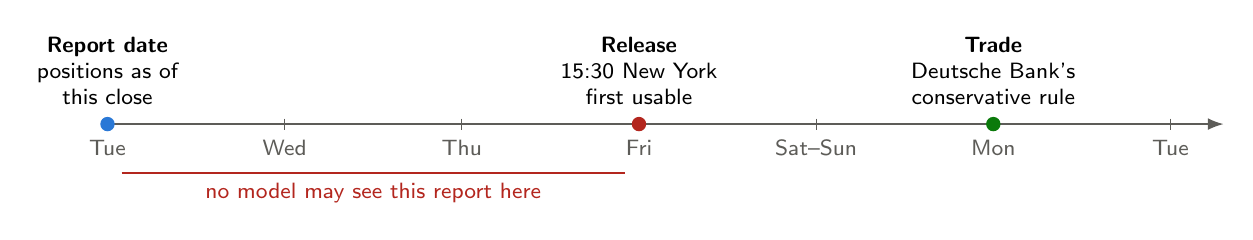
\begin{tikzpicture}[x=2.25cm,y=1cm,font=\sffamily\footnotesize]
\draw[-{Latex},muted,line width=0.6pt] (0,0) -- (6.3,0);
\foreach \x/\l in {0/Tue,1/Wed,2/Thu,3/Fri,4/Sat--Sun,5/Mon,6/Tue}{\draw[muted] (\x,0.07)--(\x,-0.07); \node[below,text=muted] at (\x,-0.08) {\l};}
\fill[longc] (0,0) circle (2.6pt);
\node[above,align=center] at (0,0.12) {\textbf{Report date}\\positions as of\\this close};
\fill[warnc] (3,0) circle (2.6pt);
\node[above,align=center] at (3,0.12) {\textbf{Release}\\15:30 New York\\first usable};
\fill[okc] (5,0) circle (2.6pt);
\node[above,align=center] at (5,0.12) {\textbf{Trade}\\Deutsche Bank's\\conservative rule};
\draw[thick,warnc] (0.08,-0.62) -- (2.92,-0.62);
\node[below,text=warnc] at (1.5,-0.62) {no model may see this report here};
\end{tikzpicture}
\caption{The weekly timing rule. Entry prices come from the Tuesday close. Knowledge starts on Friday. Deutsche Bank's FX Cookbook then trades on Monday, a delay of 4 business days.}
\label{fig:timing}
\end{figure}

\begin{decision}
\textbf{History:} use \code{publish_time()}, which assumes the normal Friday release. \textbf{Live:} store the time your job first saw each row and use that. Reports can arrive late, for example in a US government shutdown. A fixed rule would then leak information.
\end{decision}

\subsection{Market data}

\textbf{Open interest.} Use one of two modes and record which one.
\begin{itemize}
\item \textbf{Aggregate mode} sums all expiries. Use it for bond, equity, FX and energy futures. On report dates, it should equal the CFTC figure. It matched on \the\numexpr 25-2\relax{} of \ApiOiDates{} dates in the workbook.
\item \textbf{Per-expiry mode} treats each expiry as its own contract. Use it for rate strips such as SOFR. The Morgan Stanley note speaks of ``individual contract charts'', but it does not define a contract.
\end{itemize}

\textbf{VWAP.} Use the best source you have, and store which one you used.
\begin{enumerate}
\item Exchange trades: $\sum_j p_j v_j / \sum_j v_j$ over the session.
\item Intraday bars: the same sum over bars. Use \code{vwap_from_bars}.
\item Typical price: the mean of whichever of $H$, $L$ and $C$ exist, as the 2018 workbook used. This is a fallback only.
\end{enumerate}

\textbf{Rolls.} A raw front-contract price jumps at each roll. That jump creates false entry prices and false price changes. Back-adjust so the latest price stays true and earlier prices shift by each roll gap:
\[
P^{\text{adj}}_t \;=\; P_t + \sum_{r \,:\, r > t} g_r, \qquad g_r = P^{\text{new}}_r - P^{\text{old}}_r .
\]
The old code took adjusted closes (its argument type is \code{ADJ_CLOSE_SERIES}). The 2018 workbook did not. Use \code{back_adjust}. Per-expiry mode needs no adjustment.

\subsection{Data checks to run before any method}

These checks caught real faults in the workbook. Stop the job if a check marked ``stop'' fails.

\small
\begin{tabularx}{\linewidth}{@{}LlL@{}}
\toprule
Check & Action & What the workbook showed \\
\midrule
TFF and legacy identities: long side plus spreads equals open interest & stop & No failures on TY \\
A week missing from the CFTC series & stop & 11 Nov 2014 is missing from the sheet. The test files keep this gap on purpose. \\
Duplicate key in \code{options_eod}: date, expiry, strike, type & stop & Not in the workbook \\
Close outside the high--low range & flag & \QcOutside{} of \QcRows{} rows \\
High equals low & flag & \QcEqual{} rows \\
High or low missing & flag & \QcMissingRange{} rows \\
Volume missing & flag & \QcMissingVolume{} row \\
Volume collapses against its 60-day median & flag & \QcCollapse{} rows under 200,000 around the September and December rolls \\
\bottomrule
\end{tabularx}
\normalsize

The volume faults matter. The sheet pairs total open interest with front-contract volume, and that volume dies before each roll. So never weight by front-contract volume alone.

\subsection{Tables to store}

\small
\begin{tabularx}{\linewidth}{@{}lX@{}}
\toprule
Table & Columns \\
\midrule
\code{contracts} & symbol, cftc\_code, report\_for\_traders, asset\_class, dollars\_per\_point, mode \\
\code{cftc_weekly} & report, basis, code, report\_date, first\_seen, then one column per canonical field \\
\code{market_daily} & symbol, date, close, adj\_close, high, low, volume, open\_interest, vwap, vwap\_source \\
\code{options_eod} & date, root, expiry, strike, is\_call, forward, implied\_vol, abs\_delta, open\_interest, volume \\
\code{trades} & symbol, time, price, size \\
\bottomrule
\end{tabularx}
\normalsize

% ==================================================================
\section{The ledger: the engine behind every Pain method}\label{sec:ledger}
% ==================================================================

\textbf{Build this first. P1, P2 and P4's matched view all run on it.} A ledger answers one question: of the positions added inside this window, how much is still open, and at what entry price?

\subsection{The algorithm}

Inputs are one window of dates, a signed change $c_t$ for each date, and an entry price $e_t$ for each date. Replay the window from the oldest date.

\begin{enumerate}
\item Start with an empty list of lots.
\item If $c_t > 0$, add a lot with gross $c_t$, open $c_t$ and entry $e_t$.
\item If $c_t < 0$, set the request $R = -c_t$ and the available total $A = \sum_i o_i$.
\item Remove $\min(R, A)$ from the open lots under the chosen rule.
\item Record $R - \min(R, A)$ as \textbf{unmatched}. It means the reduction hit positions older than the window.
\item Rebuild from empty for every as-of date. Do not update yesterday's ledger.
\end{enumerate}

\sublabel{The removal rules}
\small
\begin{tabularx}{\linewidth}{@{}lXl@{}}
\toprule
Rule & What it does & Source \\
\midrule
\code{pro_rata} & Every lot loses the same share: $o_i \leftarrow o_i - \min(R,A)\, o_i / A$, with $A$ fixed for the whole pass. & Morgan Stanley 2014, June 2015 emails \\
\code{fifo} & Oldest lots go first. & 2018 deck, page 16 \\
\code{low_price_first} & Lowest entry prices go first. & 2018 function text \\
\bottomrule
\end{tabularx}
\normalsize

\textbf{Use \code{pro_rata}.} Two independent sources describe it, and it is the only rule argued for in writing. The June 2015 email thread's reason was that you know positions are closing, but not which ones. Any other split would be arbitrary. Figure~\ref{fig:rules} shows why this choice matters.

\begin{figure}[ht]
\centering
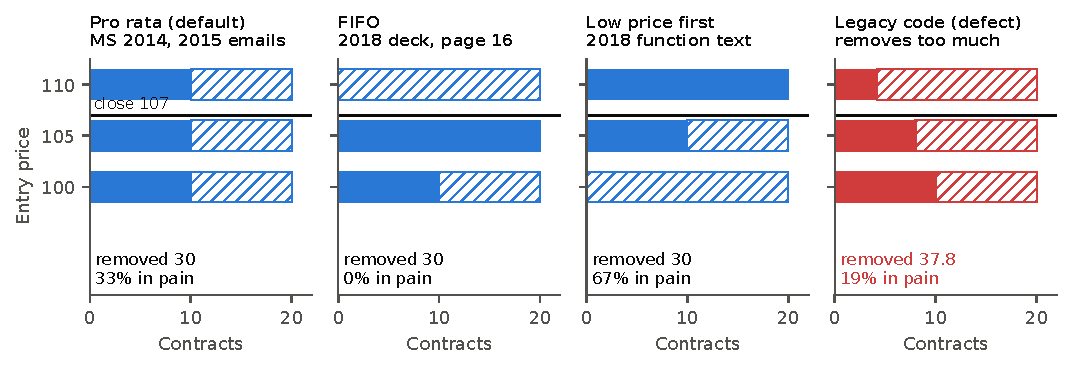
\includegraphics[width=\linewidth]{figures/rules.pdf}
\caption{The removal rule changes the answer. All four panels start from the same market: 20 contracts added at 110, then 100, then 105, then a cut of 30. Solid is still open. Hatched is removed. The pain share is the open amount above the 107 close. It runs from 0\% to 67\% across the three stated rules. The legacy code also removes \LegacyRemoved{} instead of 30.}
\label{fig:rules}
\end{figure}

\begin{checkbox}
Lots 20, 20, 20 at 110, 100, 105, then a cut of 30. Pro rata leaves 10, 10, 10. FIFO leaves 0, 10, 20. Low price first leaves 20, 0, 10. Every rule removes exactly 30.
\end{checkbox}

\sublabel{Three invariants. Check them on every run.}
\begin{enumerate}
\item Each lot satisfies $0 \le o_i \le g_i$.
\item Gross minus removed equals open.
\item Requested equals removed plus unmatched.
\end{enumerate}
\code{Ledger.check()} raises an error when any of them fails. The legacy code fails the second one.

\subsection{Conventions used by every method}\label{sec:conv}

Use these unless a method says otherwise. They make two builds agree to many decimals.

\small
\begin{tabularx}{\linewidth}{@{}P{0.26\linewidth}L@{}}
\toprule
Item & Convention \\
\midrule
Rolling window & Includes today. Return no value until the window is full. \\
Standard deviation & Sample form, dividing by $n - 1$. \\
Z-score & $(x_t - \text{mean}) / \text{std}$ over the same window, today included. \\
Lengths & 1, 3, 6 and 12 months are 21, 63, 126 and 252 trading days. A year of weekly data is 52 rows. \\
Half-life $h$ & Weight $\alpha = 1 - 0.5^{1/h}$. \\
Span $n$ & Weight $\alpha = 2/(n + 1)$. \\
Exponential mean & $m_0 = x_0$, then $m_t = \alpha x_t + (1 - \alpha) m_{t-1}$. \\
Exponential std & Use weights $w_0 = (1-\alpha)^t$ and $w_i = \alpha (1-\alpha)^{t-i}$. With $W_1 = \sum w_i$ and $W_2 = \sum w_i^2$, the variance is $\frac{W_1^2}{W_1^2 - W_2} \cdot \frac{\sum_i w_i (x_i - m_t)^2}{W_1}$. \\
Pandas equivalent & \code{ewm(halflife=h, adjust=False).mean()} and \code{.std()}. \\
Least squares & Include an intercept. \\
\bottomrule
\end{tabularx}
\normalsize

% ==================================================================
\section{The Pain methods}\label{sec:pain}
% ==================================================================

\method{P1}{Morgan Stanley Pain Trade Monitor}{\Specified{} The source is a 16 October 2014 sales note. Its one page prints no output value, so nothing exists to match. P5 is the owner's simpler reading of the same idea.}

\textbf{What it answers.} Of the positions opened in the last 30 trading days, how much is offside now?

\sublabel{Inputs, per contract}
$C_t$ close. $V_t$ daily VWAP. $O_t$ open interest. $M$ multiplier. $F_T$ USD per unit of quote currency on the as-of date $T$.

\sublabel{Steps}
\begin{enumerate}
\item Compute $\Delta C_t = C_t - C_{t-1}$ and $\Delta O_t = O_t - O_{t-1}$.
\item Label each day with Table~\ref{tab:cases}. All of the open-interest change goes to one side.
\item Take the last $N = 30$ daily changes. This needs 31 rows of levels.
\item Replay the long changes through the ledger, with entry $V_t$ and the rule \code{pro_rata}.
\item Replay the short changes through a second ledger in the same way.
\item Set the test level to the as-of close $C_T$.
\item Compute the outputs below.
\item Rank contracts by $\text{Off}/O_T$, largest first, separately for longs and shorts.
\end{enumerate}

\begin{table}[ht]
\centering\small
\caption{The four cases. The note states the idea. It does not print this table, but only this mapping fits its words.}\label{tab:cases}
\begin{tabular}{@{}lll@{}}
\toprule
& $\Delta O_t > 0$ & $\Delta O_t < 0$ \\
\midrule
$\Delta C_t > 0$ & New longs: add to longs & Shorts covered: remove from shorts \\
$\Delta C_t < 0$ & New shorts: add to shorts & Longs taken off: remove from longs \\
\bottomrule
\end{tabular}
\end{table}

\sublabel{Outputs, per side}
\begin{align*}
\text{Off}_{\text{long}} &= \sum_{i\,:\,e_i > C_T} o_i, \qquad \text{Off}_{\text{short}} = \sum_{i\,:\,e_i < C_T} o_i, \\
\text{share of new} &= \frac{\text{Off}}{\sum_i o_i}, \qquad \text{share of open interest} = \frac{\text{Off}}{O_T}, \qquad \text{USD offside} = \sum_{i \text{ offside}} o_i\, e_i\, M\, F_T .
\end{align*}

\begin{decision}
\begin{itemize}[leftmargin=*]
\item \textbf{Price change:} close to close. The note says only ``price change''.
\item \textbf{No change:} if $\Delta C_t = 0$ or $\Delta O_t = 0$, make no entry and log the day.
\item \textbf{Exact ties:} a lot entered exactly at $C_T$ is not offside.
\item \textbf{Denominators:} use contracts, not dollars, for the share of new. Report shares as fractions. If a side has no open lots, return no reading.
\item \textbf{Older positions:} a reduction larger than the ledger is capped. Publish the excess as \code{unmatched}.
\item \textbf{Rate strips:} the note's notional formula gives price times multiplier. For a SOFR contract that is far below its \$1 million face. Rank on the share of open interest, which this does not affect.
\end{itemize}
\end{decision}

\sublabel{Worked example: follow this by hand once}
Use a seven-day window, $M = 1{,}000$ and $F_T = 1$.
\begin{center}\small
\begin{tabular}{@{}rrrrrrl@{}}
\toprule
Day & Close & VWAP & Open interest & $\Delta C$ & $\Delta O$ & Label \\
\midrule
\rowsinput generated/p1_toy.tex 
\bottomrule
\end{tabular}
\end{center}

Longs: days 1 and 2 add 100 at 100.6 and 60 at 101.6. Day 4 removes 40 from 160, a quarter of each lot. That leaves 75 and 45. Shorts: day 3 adds 50 at 101.7. Day 5 covers 20, leaving 30. Day 6 adds 40 at 101.2. Day 7 covers 10 from 70, one seventh of each, leaving 25.714 and 34.286.

\begin{figure}[ht]
\centering
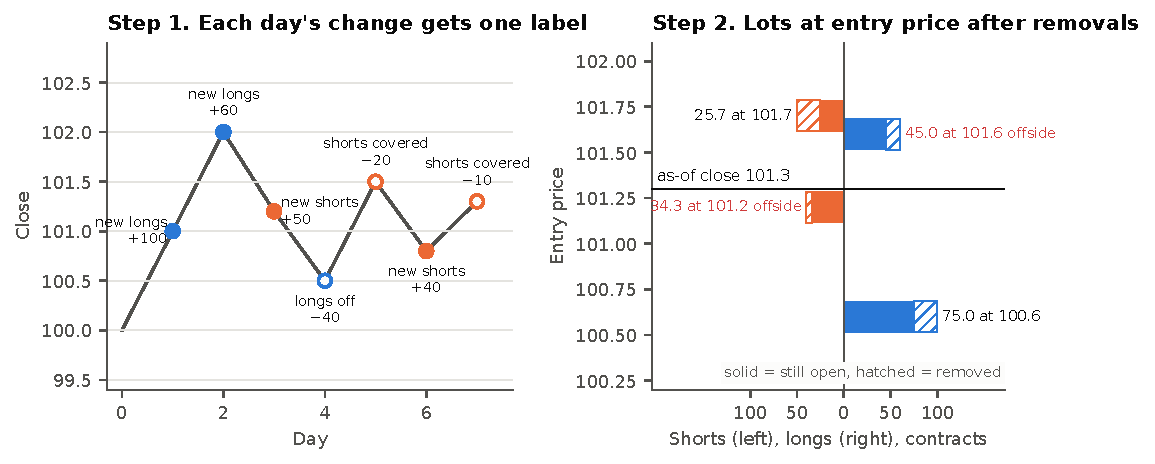
\includegraphics[width=\linewidth]{figures/ledger.pdf}
\caption{How P1 works. Left: filled markers add a position and open markers remove one. Blue is the long book. Orange is the short book. Right: the resulting lots. A long is offside above the close line. A short is offside below it. Red text marks the two offside lots.}
\label{fig:ledger}
\end{figure}

\begin{checkbox}
Toy example at close 101.3. Long offside 45, which is \ToyLongNew{} of new longs and \ToyLongOI{} of open interest, or \$\ToyLongUSD. Short offside \ToyShortOff, which is \ToyShortNew{} of new shorts and \ToyShortOI{} of open interest, or \$\ToyShortUSD.

Real TY data, 22 January 2015, typical price as the VWAP fallback, $N = 30$. Long open \TyLongOpen, offside \TyLongNew. Short open \TyShortOpen, offside \TyShortNew. Unmatched: \TyLongUnmatched{} long and \TyShortUnmatched{} short. These pin down the code. They are not market truth, because the workbook's high and low fields are unreliable.
\end{checkbox}

\begin{figure}[ht]
\centering
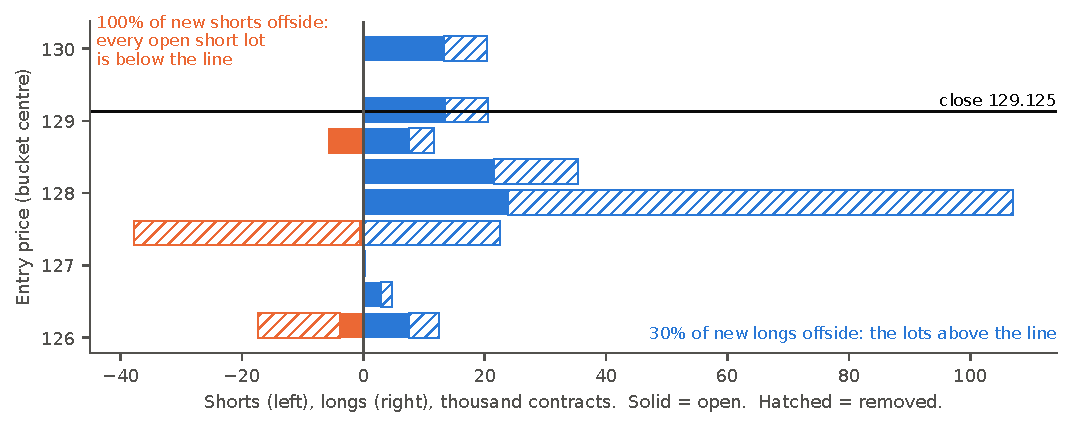
\includegraphics[width=\linewidth]{figures/ty_ladder.pdf}
\caption{P1 on real TY data at 22 January 2015, grouped into ten price buckets for reading. This is the chart to reproduce on your screen. Compute the signal from lots, not from buckets.}
\end{figure}

\begin{warnbox}[Eurodollars]
Code \code{132741} stops on 13 June 2023. Use \code{134741} (SOFR-3M) for live work. Nothing in the note says it is the document the thread refers to. It is the closest match found.
\end{warnbox}

% ------------------------------------------------------------------
\method{P2}{PortfolioStrat method, corrected}{\Specified{} Rules from the June 2015 emails, with the defects of P3 removed. No source output exists for the corrected formula. The deck's line is the legacy one, as P3 shows.}

\textbf{What it answers.} For one trader group in one market, what share of the positions opened in the window sits at a losing entry price?

\textbf{Why not P1?} P1 infers the side from price and open interest. P2 reads the side directly from the CFTC, at the cost of weekly data.

\sublabel{Inputs}
One weekly CFTC field, for example \code{lev_money_long} from TFF or \code{money_mgr_long} from the disaggregated report. The daily adjusted close. A window of $N$ trading days.

\sublabel{Steps}
\begin{enumerate}
\item Put the weekly field on the daily calendar. The change lands on its report date. All other days have zero change. If the report date is not a trading day, use the next trading day.
\item For each as-of date $T$, take the last $N$ daily rows of change. Compute changes on the full series first.
\item Zero any change from a report not yet released on $T$. This is what removes the old look-ahead.
\item Replay them through the ledger. The entry price is the close on the change date. Use \code{pro_rata}.
\item Compute the share in pain with $L = C_T$:
\[
\text{long field:}\;\; \frac{\sum_{i: e_i \ge L} o_i}{\sum_i o_i}, \qquad\qquad \text{short field:}\;\; \frac{\sum_{i: e_i \le L} o_i}{\sum_i o_i} .
\]
\item Build the ladder chart if you want one. For each ratio $r \in \{0.5, 0.6, \dots, 1.5\}$, sum the open lots with $e_i \ge r\, C_T$. \textbf{The value must fall as $r$ rises.}
\item Build the old bucket chart if you want one. Use ten equal buckets from the window's low to its high. Show gross, removed and open in each.
\end{enumerate}

\sublabel{Choose the window}
\begin{center}\small
\begin{tabular}{@{}lll@{}}
\toprule
Rows & Where it comes from & Use \\
\midrule
30 & Function default and the old screen & Only to rebuild the 2015 screen. It holds about six reports. \\
90 & Function description & Only to rebuild a saved workspace. \\
126 & ``Last six months'' in the 2018 deck & \textbf{Default for signals.} \\
\bottomrule
\end{tabular}
\end{center}

\begin{decision}
\begin{itemize}[leftmargin=*]
\item \textbf{Short fields:} the sources show only long examples for the signal. Pain for a short is below the price, so the test flips.
\item \textbf{Ties:} ``at or above'' follows the title of the deck's chart. So P2 counts a lot exactly at the price, and P1 does not. Keep this difference.
\item \textbf{Gross} covers all lots in the window, not only those in pain.
\item \textbf{Empty ledger:} when no lots remain open, return no reading. Do not return zero.
\item \textbf{Weekly path:} a week's whole change lands on Tuesday's close. That is the sources' rule, and it hides the path inside the week.
\end{itemize}
\end{decision}

\begin{warnbox}[Two outputs share one description]
The deck says the output is the percent of open positions initiated above the price. The old \code{PCT_OPEN} code returns something else: open divided by gross, among lots at or above the price. That is a survival share. For a short field, the same test looks at lots at or below the price. Both are in the code as \code{share_in_pain} and \code{pct_open_code}. On TY leveraged-fund longs, with the release rule off, they read \PtwoShare{} and \PtwoCode. Trade the first. Use the second only to explain old output. The deck's chart is the second output. On 30 rows of combined-report data it stays inside the digitised line's band for 80\% of dates, and reads the printed 1.00 on 30 January 2018. The first output reads 0.26 there.
\end{warnbox}

\begin{checkbox}
TY \code{lev_money_long}, $N = 90$, as of 22 January 2015. With the release rule off (\code{respect_release=False}, to match old output): gross \PtwoGross, open \PtwoOpen, unmatched \PtwoUnmatched, share in pain \PtwoShare. With the rule on, the share is \PtwoLive, because the 20 January report is not out until 23 January. That shows how much the rule matters. For \code{asset_mgr_long} with $N = 60$ and the rule off, no lots remain open, so the reading is empty.
\end{checkbox}

% ------------------------------------------------------------------
\method{P3}{PortfolioStrat legacy code, defects kept}{\Verified{} Exact port of \code{functions.py}, lines 961 to 1050. Use it to explain old output, never for new signals.}

\sublabel{The removal loop as written}
Ten equal buckets run from the window's low to its high. A bucket's label is its lower edge. A price goes in bucket $\lfloor (p - \text{low}) / \text{width} \rfloor$, and the top price goes in the last bucket. Each bucket keeps gross $G_b$ and liquidated $Q_b$, and net starts at zero. An addition raises both $G_b$ and net. Changes come from the full series, before the window is cut. Build each label as low $+\, b \times$ width, so exact ties behave the same. A reduction is ignored while net is zero. On a reduction of size $x$, the code walks the buckets from the lowest price:
\[
\text{take}_b = \min\!\Big(\frac{G_b - Q_b}{\text{net}}\, x,\; G_b - Q_b\Big), \qquad Q_b \mathrel{+}= \text{take}_b, \qquad \text{net} \mathrel{-}= \text{take}_b .
\]
\textbf{Net shrinks inside the loop.} So later buckets lose more, and the total passes $x$. With 20 in each of three buckets and $x = 30$, the takes are 10, then 12, then 15.79. The total is \LegacyRemoved{}. The buckets lose 50\%, 60\% and 79\%.

\sublabel{What the function returns at level $L$, for condition \code{>=}}
\code{PCT_OPEN} is $\sum_{b: \text{label}_b \ge L} (G_b - Q_b) \,/\, \sum_{b: \text{label}_b \ge L} G_b$, or zero if the bottom is zero. \code{OPEN} is the sum of $G_b - Q_b$ over buckets where that same open amount is at least $L$. \code{GROSS} and \code{CLOSED} work the same way on their own amounts. For \code{<=}, flip both tests. For \code{==}, it interpolates linearly across bucket labels. The function rolls over $N$ daily rows and rebuilds each time.

\sublabel{Defects found}
\small
\begin{longtable}{@{}P{0.31\linewidth}P{0.64\linewidth}@{}}
\toprule
Defect & Evidence and effect \\
\midrule
\endhead
Removes too much & Net shrinks inside the loop. It removes \LegacyRemoved{} when asked for 30. \\
Compares size with price & Lines 1003 and 1009 test the bucket's quantity against the price level for \code{OPEN}, \code{GROSS} and \code{CLOSED}. See Figure~\ref{fig:ladder}. \\
\code{PCT_OPEN} is a survival share & It returns open over gross above the level. The deck describes a share of all open positions. \\
Three descriptions, none correct & The 2018 text says lower prices are liquidated fastest. The deck says FIFO. The code removes the largest share from the highest prices, by bucket order and not by date. \\
Buckets blur the test & A bucket is labelled by its lower edge. A lot above the level but inside its bucket is missed, an error of up to one bucket width. \\
Flat window fails & When the low equals the high, the bucket width is zero and the function fails. \\
Look-ahead & A change is used from its report date, three days before release. \\
Python 2 only & \code{xrange} and positional label access. The port in \code{pain.py} fixes these two syntax points and nothing else. \\
\bottomrule
\end{longtable}
\normalsize

\begin{figure}[ht]
\centering
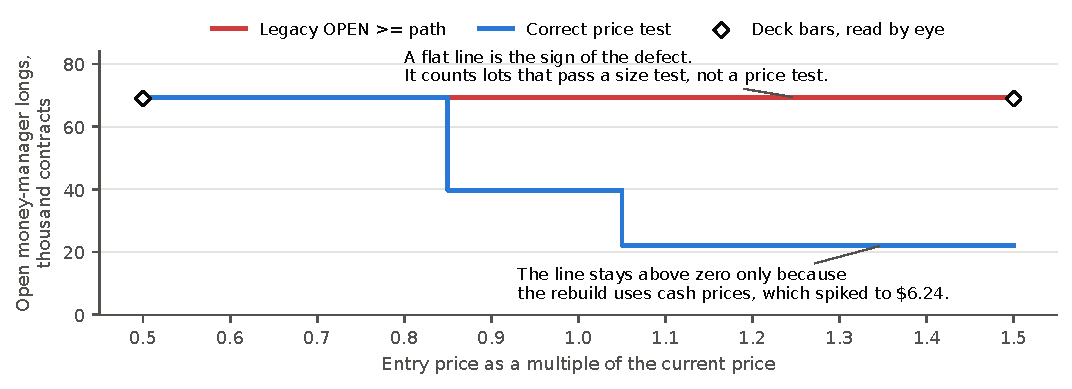
\includegraphics[width=\linewidth]{figures/ladder.pdf}
\caption{The natural gas ladder in the 2018 deck very likely carried the size-versus-price defect. Real CFTC money-manager longs through the legacy path give \NgLegacy{} contracts at every row. The deck's bars, read by eye, also sit flat near 69,000. A correct test must step down as the price multiple rises, and the blue line does. The rebuild uses Henry Hub cash prices because I have no futures history. The saved workspace is not in evidence, so this is strong evidence and not proof.}
\label{fig:ladder}
\end{figure}

\begin{checkbox}
Changes $[20, 20, 20, -30, 0]$ at prices $[100, 105, 110, 102, 100]$ give removed \LegacyRemoved. Changes $[10, 10, -5, 0]$ at $[100, 110, 105, 100]$ give removed 5.357. Natural gas ladder as of 30 January 2018, money-manager longs, 126 rows: \NgLegacy{} at every ratio. Outside check: the deck's line is this output. On 30 rows of combined-report data it stays inside the digitised line's band for 80\% of dates and reads the printed 1.00. This comes from 50 variants, with one unfitted confirmation, on a coarse screenshot.
\end{checkbox}

% ------------------------------------------------------------------
\method{P4}{Activity by trade price}{\Verified{} From the June 2015 email thread. This is not a Pain measure. The thread calls it an intermediate step.}

\textbf{What it answers.} How much buying and selling happened at each price? It places every change at the price of the day it happened. It does not match exits to entries.

\sublabel{Steps}
\begin{enumerate}
\item Compute the daily change of the long series and of the short series.
\item Split each into additions and removals, and group by that day's price.
\item Compute buys as longs added plus shorts taken off. Compute sells as shorts added plus longs taken off.
\end{enumerate}

\begin{checkbox}
The thread's worked example: prices 100, 105, 110, 105, 110 with longs and shorts both 0, 6, 6, 3, 0. At 105: longs added 6, longs off 3, buys 9, sells 9. At 110: longs off 3, buys 3, sells 3. The entry-matched view of the same data is a ledger. It shows one lot at 105, gross 6, removed 6, open 0, which matches the Pain Monitor block of the Google Sheet.
\end{checkbox}

% ------------------------------------------------------------------
\method{P5}{The owner's workbook reading of P1}{\Verified{} All seven formula columns match every cached cell, with a largest gap below $10^{-13}$. Verified means the code matches the workbook. It does not verify P1 against Morgan Stanley.}

\textbf{What it answers.} Is the market's net new position above or below water against a rolling average price? This workbook is the owner's own reading of the Morgan Stanley Pain idea. The file was last saved in January 2015 and emailed in 2018.

\sublabel{How it differs from P1}
\begin{center}\small
\begin{tabularx}{\linewidth}{@{}lXX@{}}
\toprule
& P1 & P5, the workbook \\
\midrule
Positions & Separate long and short books at once & One net number, so one side at a time \\
Entry price & Each day's VWAP, for days that add positions & One blended price over 30 rows, including days when positions fell \\
Weights & The open interest added & All volume \\
Output & Contracts and dollars offside & A price gap only, with no size \\
\bottomrule
\end{tabularx}
\end{center}

On the workbook's 95 usable TY days, they agree on whether most of the position is under water on 73.7\% of days. The correlation is 0.66. P1's larger book matches the workbook's side on only 48.4\% of days, because P1 can hold large longs while net open interest falls. The workbook's side can also flip on a small change: it reads Short on 20 January 2015 and Long the next day. Rerun with \code{scripts/compare_p1_workbook.py}. This is one contract over about five months, so it shows how they differ, not which is right. Keep both. Neither has an out-of-sample test yet.

\sublabel{Columns, for each row $t$}
\begin{align*}
G_t &= \text{mean of the available } H_t, L_t, C_t && \text{typical price} \\
J_t &= O_t - O_{t-1} && \text{change in open interest} \\
M_t &= \frac{\sum_{s=t-29}^{t} K_s G_s}{\sum_{s=t-29}^{t} K_s} && \text{called VWAP: 30 rows of volume } K \\
N_t &= \sum_{s=t-28}^{t} J_s && \text{net new position: 29 changes} \\
\text{Side}_t &= \text{Long if } N_t > 0, \text{ else Short} \\
P_t &= G_t - M_t && \text{over or under water}
\end{align*}

Both windows expand from the first row until they fill. A missing volume counts as zero. The sheet stops at $P_t$. I add the flag \code{underwater}: long with $P_t < 0$, or short with $P_t > 0$.

\begin{warnbox}[Faults in the workbook. Do not copy them.]
\begin{itemize}[leftmargin=*]
\item \code{M} is not a daily VWAP. It is a rolling weighted mean of typical price, so it differs from P1's $V_t$.
\item \code{Sheet1} columns B and C use \code{VLOOKUP} on the wrong column, without an exact match, and with the wrong column number. Every row returns the last row's values.
\item \code{Sheet1} column K adds dealer shorts and non-commercial longs to long fields from another report. It is not a total of longs.
\item Column L holds an error value on 18 December 2014, because volume is missing there.
\end{itemize}
\end{warnbox}

\begin{checkbox}
Last row, 22 January 2015: VWAP \WbVwap, net new \WbNet, side \WbSide, over or under \WbOver.
\end{checkbox}

% ==================================================================
\section{The positioning indicators}\label{sec:ind}
% ==================================================================

\textbf{Next action: build I1, I2 and I3 first. They need only the CFTC feed, and all three are verified.} These methods measure how stretched positions are. None estimates entry prices.

\method{I1}{Net position as a share of open interest}{\Verified{} Deutsche Bank's weekly note, May 2017.}

\begin{enumerate}
\item Take non-commercial longs and shorts from the legacy futures-only report.
\item Compute net $= $ longs $-$ shorts, and $100 \times$ net $/$ open interest.
\item Add the 52-week high, low and median of that share. The note's first figure shows them.
\end{enumerate}

\begin{checkbox}
Week to 9 May 2017, against the note's words. TY net \DbTyNet{} (229K), up \DbTyChg{} (49K). WN net \DbWnNet{} ($-$108K), change \DbWnChg{} (19K more short). FV change \DbFvChg{} (45K more short). US change \DbUsChg{} (pared 4K). Eurodollar change \DbEdChg{} (90K more short), share \DbEdPct\% (24\%).
\end{checkbox}

% ------------------------------------------------------------------
\method{I2}{Goldman Sachs sentiment index}{\Verified{} Sources: Global Viewpoint 12/17 (July 2012) and Global Markets Daily (18 July 2016).}

\textbf{What it answers.} Where does today's net position sit between its 3-year low and high?

\begin{enumerate}
\item Compute net position $NP_t$ in contracts from the legacy futures-only report.
\item Over the 156 weeks ending today, including today, find the low and the high.
\item Compute $SI_t = 100\,(NP_t - \text{low}) / (\text{high} - \text{low})$.
\item Set $D^{90}_t = 1$ if $SI_t \ge 90$. Set $D^{10}_t = 1$ if $SI_t \le 10$.
\item Add a counter of consecutive weeks in the current extreme. It captures how fresh the extreme is.
\end{enumerate}

\begin{figure}[ht]
\centering
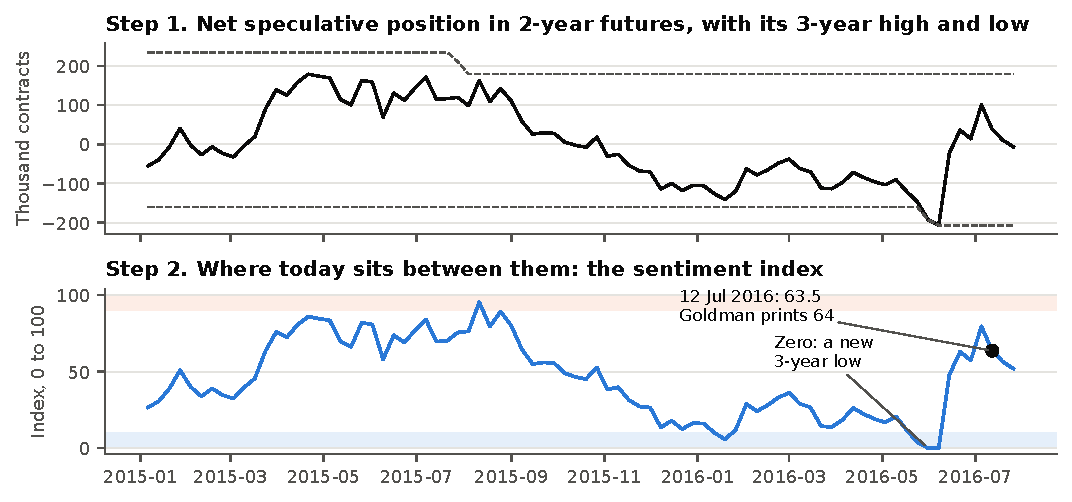
\includegraphics[width=\linewidth]{figures/si.pdf}
\caption{How to read the index. The top panel is the raw net position and its 3-year bounds. The bottom panel asks how far today sits between them. Shaded bands are the extreme zones. A reading of zero means a new 3-year low in net position.}
\end{figure}

\sublabel{The two regressions Goldman runs}
\[
R_{t+k} = \beta_0 + \beta_1 SI_t + \varepsilon_t, \qquad\qquad
R_{t+k} = \beta_0 + \beta_1 SI_t + \beta_2 D^{90}_t + \beta_3 D^{10}_t + \varepsilon_t .
\]
\begin{itemize}
\item \textbf{FX (2012):} $R$ is the percent change in the currency against the dollar, for $k = 1, \dots, 10$ weeks. The sample runs from January 1999 to July 2012.
\item \textbf{Treasuries (2016):} $R$ is the change in yield, for $k = 2, 4, 8$ weeks. The sample runs from December 2001 to June 2016. A positive $\beta$ means a higher index goes with higher yields.
\item \textbf{Standard errors:} Newey-West, because the returns overlap. Use \code{si_regression}.
\end{itemize}

\begin{decision}
The sources say ``3-year'' and give no lag count. Use 156 weeks. Set the Newey-West lag equal to $k$. Date a reading by the report date, then apply the release rule for any test.
\end{decision}

\begin{checkbox}
EUR on 24 July 2012: \SiEur{} (Goldman prints 18.9\% in its 31 July note). EUR zero readings in May and June 2012: \SiEurZero{} weeks (Goldman says four). 2-year on 12 July 2016: \SiTwo{} (Goldman prints 64). 10-year on that date: \SiTen{} (Goldman calls it the longest in three years).

\textbf{One gap:} Goldman says the 2-year sat at zero for three weeks around end-May 2016. I get \SiTwoZero{} weeks at zero. The week before reads 3.8.
\end{checkbox}

Goldman's finding is worth keeping in mind. In 2016 extreme readings worked as a contrarian signal for 2-year and 5-year futures, but not for 10-year. In 2012, stretched EUR positioning led the currency for about a month instead of reversing it.

% ------------------------------------------------------------------
\method{I3}{Deutsche Bank scaled positioning}{\Verified{} Sales note, 15 May 2017. The note gives only the end points, so I tested three formulas against its chart.}

\textbf{What it answers.} How large is today's net position against the largest long and largest short of the last four years?

\begin{enumerate}
\item Compute net contracts for one TFF group, futures only: leveraged funds or asset managers.
\item Over the last 209 weekly rows, which is four years counting both end dates, find the largest net long $U$ and the largest net short $W$, as a positive number.
\item If net is positive, the score is $10 \times \text{net} / U$. If net is negative, it is $10 \times \text{net} / W$. If net is zero, the score is zero.
\end{enumerate}

\begin{checkbox}
I read 22 values off the note's chart for 9 May 2017 and rebuilt them. Mean error \DbScaledMae{} points, largest \DbScaledMax. A min-max scale gives a mean error of about 2.1, so it is wrong. Scaling by the largest absolute value gives 0.32.
\end{checkbox}

\begin{center}\small
\begin{tabular}{@{}lrrrr@{}}
\toprule
Market & Leveraged, chart & Leveraged, rebuilt & Asset mgr, chart & Asset mgr, rebuilt \\
\midrule
\rowsinput generated/db_scaled.tex 
\bottomrule
\end{tabular}
\end{center}

% ------------------------------------------------------------------
\method{I4}{One-standard-deviation rule}{\Partial{} Goldman, January 2019, as a benchmark inside its OPI report. The sample and base rate are likely pinned. The position recipe is not.}

\begin{enumerate}
\item Sum net non-commercial contracts in TU, FV, TY and US from the legacy combined report. This is the closest recipe found, not Goldman's confirmed one.
\item Score it with the mean and standard deviation of June 2009 to January 2018.
\item A score of $-1$ or lower is a buy signal. A score of $+1$ or higher is a sell signal.
\item Measure hits against the 4-week change in Tuesday \code{DGS10}. Count a zero change as a rally.
\end{enumerate}

\begin{warnbox}[Not matched]
Goldman prints a 53\% base rate, 63\% buy and 48\% sell. The sample above gives a base rate of \SdRally, and it fits the unconditional curve in Exhibit 1 (RMSE 0.025). No position recipe of 63,893 tried reproduces buy and sell inside that sample. This recipe gives \SdBuy{} and \SdSell. Tuesday \code{DGS10} also spans less than the chart's range, so Goldman's yield series or timing differs. Treat this rule as a simple benchmark only.
\end{warnbox}

\begin{warnbox}[Look-ahead]
The frozen mean and standard deviation use the whole sample, so these hit rates are in-sample. After the sample, in a research run with a scale frozen on January 2007 to June 2018, the rule said buy in 282 of 386 weeks. Its buy hit rate was 43\%, equal to the 43\% base rate.
\end{warnbox}

% ------------------------------------------------------------------
\method{I5}{Goldman filtered position and residual}{\Verified{} Global Rates Insights, 9 May 2019. This build tracks the weekly series drawn in Goldman's own charts at \GfChartLev{} and \GfChartAm.}

\textbf{What it answers.} Have yields moved further than the positioning of the marginal investor implies? If so, expect some reversal over six months.

\sublabel{Steps}
\begin{enumerate}
\item Use the combined futures-and-options report. Start in June 2006, and work weekly.
\item Compute net contracts by group and contract, using the table below. Add asset managers and other reportables before filtering.
\item For each contract, keep the weekly change in net only if it moves with that contract's yield. That means net selling as the yield rises, or net buying as it falls. Set the rest to zero.
\item Multiply each kept change by that week's contract DV01. Sum across contracts and divide by one million. The result $f_t$ is in \$mm per basis point.
\item Regress the weekly change in \code{DGS10}, in basis points, on $f_t$. Use June 2006 to December 2010 only, with an intercept.
\item Compute the residual for all weeks: $\text{res}_t = \Delta y_t - \alpha - \beta f_t$.
\item Sum the residual over 26 weeks. Call the sum $S_t$.
\item Compute the score $Z_t = S_t / (\sigma \sqrt{26})$. Here $\sigma$ is the standard deviation of the weekly residual over the fit window. Subtract no mean.
\item Score above $+0.25$: rally bias, long duration. Score below $-0.25$: sell-off bias, short duration. Otherwise, no view.
\end{enumerate}

\begin{center}\small
\begin{tabular}{@{}lll@{}}
\toprule
Group & Report and fields & Contracts \\
\midrule
Asset managers and others & TFF: \code{asset_mgr} plus \code{other_rept} & TY, US \\
Leveraged funds & TFF: \code{lev_money} & TU, FV, TY, TN, US, WN \\
Specs & Legacy: \code{noncomm} & TU, FV, TY, TN, US, WN \\
\bottomrule
\end{tabular}

\medskip
\begin{tabular}{@{}lcccccc@{}}
\toprule
Contract & TU & FV & TY & TN & US & WN \\
\midrule
Yield that decides ``with the market'' & \code{DGS2} & \code{DGS5} & \code{DGS7} & \code{DGS10} & \code{DGS20} & \code{DGS30} \\
\bottomrule
\end{tabular}
\end{center}

\begin{decision}
\begin{itemize}[leftmargin=*]
\item \textbf{Late contracts:} TN and WN add nothing until they list.
\item \textbf{Yield series:} use the last value on or before the report date.
\item \textbf{Hit counts:} count weeks with a score beyond $\pm 0.25$ and a known yield change 26 weeks later.
\item \textbf{No look-ahead after the fit window:} $\alpha$, $\beta$ and $\sigma$ stay frozen, so a live score uses only past data. The DV01 file is not point-in-time, but it moves slowly.
\end{itemize}
\end{decision}

\sublabel{Build the DV01 file}
Goldman's report says only ``duration-weighted''. No public table lists DV01 per contract, so \code{./scripts/dv01/refresh.sh} builds \code{data/treasury_futures_dv01.csv} from public data. It takes about 2 minutes. Rerun it monthly, when OFR updates.
\begin{enumerate}
\item \textbf{From March 2013:} the Office of Financial Research (OFR) publishes each contract's position in notional and in 10-year equivalents. Their ratio gives each contract's duration against TY. OFR's total DV01 over total 10-year equivalents gives the TY level. All eight group-and-side series give the same level, to the cent.
\item \textbf{Before March 2013:} build each contract's deliverable basket from TreasuryDirect records. Price each bond on the FRED yield curve. Compute each conversion factor with the CME formula. The CTD has the lowest price over conversion factor. DV01 is the CTD's DV01 over its conversion factor. Scale to meet OFR over its first 26 weeks.
\end{enumerate}
The formula reproduces two published conversion factors exactly: 0.9506 and 0.8711. Over March 2013 to 2019, the bond build sits within 2 to 5\% of OFR for FV, TY, TN, US and WN, and 9\% for TU. It also catches the jump in US near the end of 2015, when the 2031 bond left the basket and the CTD became the 2036 bond.

\begin{table}[ht]
\centering\small
\caption{I5 against the report, asset managers and others unless stated. Goldman quotes the first three rows as sizes on an inverted axis, so compare their sizes. My signs are negative because buying goes with falling yields.}\label{tab:gf}
\begin{tabular}{@{}lrr@{}}
\toprule
Statistic & Goldman & This build \\
\midrule
Yield change per \$10mm/bp (bp), three groups & 17 to 18 & \GfAmSlope, \GfLevSlope, \GfSpecSlope \\
6m filtered vs 6m yield change, asset managers & about 62\% & \GfAmCorr \\
6m filtered vs 6m yield change, leveraged funds & about 49\% & \GfLevCorr \\
Next-6m correlation, specs & $-$26\% & \GfSpecFwd \\
Next-6m correlation, leveraged funds & $-$18\% & \GfLevFwd \\
Next-6m correlation, asset managers & $-$43\% & \GfAmFwd \\
Outright 6m change vs next 6m & $-$35\% & \GfOutright \\
Volatility of filtered changes, asset managers over specs & about 2/3 & \GfVolRatio \\
Size of $\pm 0.25$ score (bp) & about 15 & \GfQuarter \\
Observations, base rally rate & 620, 55.3\% & \GfTotal, \GfUncond \\
Positive residual: count, hit rate, average (bp) & 224, 74.1\%, $-$40 & \GfPosN, \GfPosHit, \GfPosAvg \\
Negative residual: count, hit rate, average (bp) & 253, 66.8\%, +21 & \GfNegN, \GfNegHit, \GfNegAvg \\
Score on 30 April 2019 & $-$0.67 & \GfLast \\
\bottomrule
\end{tabular}
\end{table}

\sublabel{How the report's hidden choices were found}
Goldman's charts are vector graphics, so the PDF holds the weekly series itself. \code{scripts/goldman_chart_check.py} reads them and writes \code{data/goldman_chart_check.json}. It stores statistics only, never the series.

\begin{itemize}
\item \textbf{The charts fix four hidden choices.} They are the combined report, the filter yields, TY and US only for asset managers, and the score scale.
\item \textbf{Weights confirm the build.} I undid the 26-week sums and fitted a weight per contract, with no DV01 input. Table~\ref{tab:gfweights} shows the fitted weights land on the real DV01 values. Asset managers load only on TY and US, in all three periods.
\item \textbf{The score rule has no fitted number.} Goldman's implied scale is \GfImplAm{} for asset managers and \GfImplSpec{} for specs. The rule gives \GfScaleAm{} and \GfScaleSpec.
\item \textbf{Tracking.} Against Goldman's charts, the score correlations are \GfChartAmZ{} for asset managers and \GfChartSpecZ{} for specs. The 6-month series reach \GfChartLev{} and \GfChartAm. Futures-only data gives \GfChartLevFut{} and \GfChartAmFut.
\end{itemize}

\begin{table}[ht]
\centering\small
\caption{Fitted weekly weight against real DV01, in dollars per contract. A dash means the contract was not listed.}\label{tab:gfweights}
\begin{tabular}{@{}llrrrrrr@{}}
\toprule
Period & Series & TU & FV & TY & TN & US & WN \\
\midrule
\rowsinput generated/gf_weights.tex 
\bottomrule
\end{tabular}
\end{table}

\textbf{What this means.} The method now reproduces. Two details remain unexplained: Goldman counts two fewer weeks, and the report gives no reason for dropping TU, FV, TN and WN from asset managers.

\begin{warnbox}[Do not trade I5]
Verified means this build matches Goldman's charts. It does not mean the signal works. From May 2019 to October 2026, with Monday entry, the asset manager correlation with the next 26-week yield change is +4\%. It was $-$27\% for 2011 to April 2019 and $-$43\% as published. The published number includes the fit period, where it reaches about $-$64\%. Random flows through the same filter also give a slope near 18 bp per \$10mm, because the filter keeps only flows that move with yields. See Section~\ref{sec:improve}.
\end{warnbox}

% ------------------------------------------------------------------
\method{I6}{Goldman options-implied position indicator}{\Partial{} Global Rates Insights, 17 January 2019. The bands, signals and hit rates reproduce from Goldman's own line. The raw OPI has not run on real markets, because I have no strike-level data.}

\textbf{What it answers.} Are option trades building bullish or bearish exposure? Big rises in call open interest against total volume read as bullish.

\sublabel{Steps}
\begin{enumerate}
\item Each day, keep the front three option expiries.
\item Keep strikes with $|K - F| \le 10$, where $F$ is the forward itself. In 0.5 steps that is up to 41 strikes.
\item For each strike, get the daily change in open interest $\Delta OI$, the volume $V$ and the delta $\delta$.
\item Compute the raw daily indicator:
\[
OAI = \frac{\sum_c \delta_c \Delta OI_c - \sum_p \delta_p \Delta OI_p}{\sum_c \delta_c V_c + \sum_p \delta_p V_p}.
\]
\item Smooth each of the four sums with a 25-day half-life, then rebuild the ratio:
\[
OPI = \frac{EMA(\sum_c \delta_c \Delta OI_c) - EMA(\sum_p \delta_p \Delta OI_p)}{EMA(\sum_c \delta_c V_c) + EMA(\sum_p \delta_p V_p)}.
\]
\item Compute bands on the OPI series. The centre is an exponentially weighted mean with a half-life of 63 days. The half-width is $k$ times the standard deviation of all OPI values to date. This standard deviation expands. Use $k = 0.85$ for TY and $k = 1.25$ for Bunds.
\item Above the upper band, sell duration. Below the lower band, buy duration. Measure hits over the next 4 weeks.
\end{enumerate}

\begin{decision}
\begin{itemize}[leftmargin=*]
\item \textbf{Deltas are absolute values.} The report does not say so. But its stated bounds need it: $-1$ means every call trade is an unwind and every put trade is new. That gives $-1$ only with positive deltas.
\item \textbf{Delta source:} Black-76 from settlement volatility, if your vendor has no delta. Use \code{black76_abs_delta}.
\item \textbf{Bands use yesterday's values,} to avoid look-ahead. The report says ``3-month half-lives''. I use 63 trading days.
\item \textbf{The band centre and width:} the report's ``exponentially weighted standard error bands'' describes only the centre. Its charts fix the width as an expanding standard deviation. An exponentially weighted width correlates only 0.906.
\end{itemize}
\end{decision}

\begin{warnbox}[The report contradicts itself]
Page 4 says a buy signal comes at the upper threshold. Its summary, its Exhibit 3 and its logic all say the opposite: a breach of the upper band is bullish positioning and a sell signal. This specification follows those three.
\end{warnbox}

\begin{checkbox}
Formula tests: OAI equals $+1$ and $-1$ at the report's two stated limits. OAI stays within those bounds on 500 random strikes. Upper-band breach gives a sell.

Band recipe against Goldman's vector charts: centre 0.9997 and 0.9998, width 0.9994 and 0.9987. Implied $k$ is 0.846 and 1.242, against printed 0.85 and 1.25. The Bund chart played no part in choosing the recipe.

From Goldman's drawn line and bands: sell and buy days 186 and 255, against 189 and 261. Hit rates 64.0\% and 72.2\%, against 64.0\% and 73.2\%. Combined 68.7\%, against 69.3\%. Likely recipe from 256 variants: start about April 2010, enter one day after the signal, and measure over 21 trading days. Means, medians, standard deviations and the 47\% base rate were not in that search, and they match too.

Raw OAI and OPI remain untested. \code{marketdb} holds no CME options. Combined minus futures-only is not a stand-in: it never beats a correlation of 0.30 across 32 variants.
\end{checkbox}

% ------------------------------------------------------------------
\method{I7}{Deutsche Bank FX Cookbook signals}{\Partial{} Quantcraft, 15 January 2019, sections 4.5 and 4.6. The rebuilt portfolios track Figure 42 at monthly correlations of 0.93, 0.82 and 0.80, with nothing fitted but the date map. COFFEE is not rebuilt, because it needs DTCC data.}

\sublabel{CFTC continuation signal}
With $l_t$ and $s_t$ the non-commercial longs and shorts,
\[
s^{\text{cont}} = \frac{L - S}{L + S}, \qquad L = \sum_{h=0}^{3} l_{t-h}, \qquad S = \sum_{h=0}^{3} s_{t-h}.
\]

\sublabel{CFTC reversal signal}
\begin{enumerate}
\item Compute the z-score of the current net position over 1, 2 and 3 months.
\item Average the three z-scores.
\item Divide by the standard deviation of daily returns over the last 6 months. Do not annualise it.
\item Multiply by $-1$. Apply no smoothing.
\end{enumerate}

\sublabel{COFFEE signal (Categorised Option Flow in Foreign Exchange)}
\begin{enumerate}
\item Each day, take DTCC-reported European options expiring in under one year, excluding those expiring today.
\item Keep absolute deltas between 0.25 and 0.75.
\item Sum call notional minus put notional over the last 4 weeks.
\item Divide by the standard deviation of those 4-week sums over the last year.
\end{enumerate}

\sublabel{Portfolios}
Time series: $w_i = \text{sign}(s_i)\,(1/\sigma_i) / \sum_j (1/\sigma_j)$. Cross section: rank the signals, go long the top half and short the bottom half, with equal weights that sum to 100\% in absolute value. In an odd pool, the middle asset gets zero. The report finds that the reversal signal works only in the cross section.

\begin{decision}
\begin{itemize}[leftmargin=*]
\item \textbf{Lengths:} 1, 2 and 3 months are 4, 8 and 13 reports. COFFEE's 4 weeks are 20 trading days. Its volatility window is 252 trading days. Reversal volatility is 126 trading days of daily returns, read at the latest day on or before the report.
\item \textbf{Timing:} trade on the Monday after release, as the report advises.
\item \textbf{Currency sign:} CFTC contracts are long the foreign currency. Rank the cross section on signals that are long the foreign currency. Flip only to express the trade as USD/XXX, for USD/CAD, USD/JPY, USD/CHF, USD/BRL and USD/MXN. Ranking after the flip breaks the match.
\item \textbf{Ruble:} keep USD/RUB until the CFTC series ends on 15 March 2022, then drop it. H.10 does not carry it. Use the Bank of Russia official rate.
\item \textbf{Volatility in time-series weights:} 21 trading days of daily returns.
\item \textbf{Windows:} a window of $N$ weeks holds the mean of the last $N$ weekly portfolios.
\item \textbf{Returns:} spot plus carry. Spot alone keeps the correlation but cuts the time-series Sharpe from 0.29 to 0.12.
\end{itemize}
\end{decision}

\begin{checkbox}
Rebuild from June 1999 to 2018, 10 currencies, weekly, with carry (\code{research/replication/i7_rebuild.py}). Correlation with Figure 42 at weekly, monthly and quarterly frequency: time-series continuation 0.84, 0.93, 0.94. Cross-sectional continuation 0.73, 0.82, 0.86. Cross-sectional reversal 0.69, 0.80, 0.81. Rebuilt gross Sharpe 0.29, 0.22, 0.41, against chart net 0.35, 0.30, 0.26. Reversal turnover is 48, 33, 21 and 7.5, against printed 56, 42, 26 and 9.4.
\end{checkbox}

\begin{warnbox}[Why I7 is not Verified, and two faults in the source]
Weekly correlation stops at 0.84. The reversal Sharpe sits well above the chart's. Before June 1999 the fit is poor, because FRED no longer serves daily Deutsche mark rates. In the source, Figure 40's cross-sectional turnover line equals Figure 41's reversal line point for point. Figure 42 prints a reversal Sharpe of 0.25, while its text and bar say 0.22.
\end{warnbox}

% ------------------------------------------------------------------
\method{I8}{JPMorgan CTA proxy}{\Partial{} Cross Asset CTA Activity Update, 30 October 2023. It points to an earlier report that is not in evidence. Choices below are mine.}

\textbf{What it answers.} Are trades at CTA execution times following the trend signal? If they are, CTAs are probably adding. If they trade against it, they are probably unwinding.

\sublabel{Part 1: the trend signal (Baz et al. 2015, as restated by Lim et al. 2019)}
\begin{enumerate}
\item For each pair $(S,L) \in \{(8,24), (16,48), (32,96)\}$, compute exponential averages of price. A time-scale $n$ has a half-life of $\log(0.5)/\log(1 - 1/n)$.
\item Set $q_t = (m_S - m_L) / \text{std}(P;\, 63 \text{ days})$.
\item Set $Y_t = q_t / \text{std}(q;\, 252 \text{ days})$.
\item Set the response $\phi(Y) = Y \exp(-Y^2/4) / 0.89$. It peaks near $Y = \sqrt{2}$, then fades.
\item Average the three responses.
\end{enumerate}

\sublabel{Part 2: the proxy}
\begin{enumerate}
\item Classify each trade as buy or sell, and sum signed contracts per minute.
\item Choose the minutes that represent CTA execution, and sum imbalance across them each day.
\item Over a rolling month, compute the correlation and the beta of imbalance on the signal.
\item Score the beta against its own history with a zero mean: $z_t = \beta_t / \sqrt{\overline{\beta^2}}$, where the average covers all betas up to today.
\end{enumerate}

\begin{decision}
\begin{itemize}[leftmargin=*]
\item \textbf{Trade classifier:} the tick rule. The report does not name one.
\item \textbf{Execution minutes:} unknown. Use \code{pick_execution_minutes} on past data, then freeze the list.
\item \textbf{Averaging:} Lim et al.\ average trend strengths in their equation but speak of averaging positions. I average positions. Check Baz et al.\ before trading. I could not download it.
\item \textbf{Month:} 21 trading days. Beta is the covariance over the variance of the signal.
\item \textbf{Signal size:} the report's signals pass 1.5, so they cannot be an average of the response, which caps at 0.96. A sum of the three responses fits better on yield proxies, with a mean gap of 0.31 against 1.10. This is a likely recipe from 16 variants. Check it against futures prices.
\item \textbf{Exponential averages:} seed with the first price, as in Section~\ref{sec:conv}.
\end{itemize}
\end{decision}

\begin{checkbox}
Formula tests only: $\phi$ peaks at $\sqrt{2}$, the beta recovers a known slope, and an uptrend gives a positive signal. The report's table to sanity-check against, 30 October 2023: TY beta 77,517 contracts, z-score 1.71, signal $-$1.78.
\end{checkbox}

% ------------------------------------------------------------------
\method{I9}{Citi FX positioning indicator}{\NotRep{} CitiFX Flows \& Positioning, 29 April 2019. It rests on Citi's private client flows.}

The indicator runs from $-$10 to +10 per currency. Its parts are below.

\begin{center}\small
\begin{tabular}{@{}ll@{}}
\toprule
Block & Inputs named in the report \\
\midrule
Leveraged & CitiFX flows, CFTC, CPAIN \\
Real money & CitiFX flows, CFTC \\
Retail & OANDA, ETFs, Japan retail \\
\bottomrule
\end{tabular}
\end{center}

\textbf{The weights are hidden.} Simple averages do not reproduce the page. USD leveraged prints 0, but its parts (1, $-$2, $-$3) average $-$1.33. The report does not define CPAIN. A public proxy can use I3 on CFTC data. Do not label that proxy as Citi's indicator.

% ------------------------------------------------------------------
\method{I10}{Morgan Stanley Bond Market Indicators}{\Partial{} Global Rates Strategy, 6 March 2015. This is a duration model, not a positioning measure. The combination rules are verified. Two inputs are not fully stated.}

\sublabel{The four factors, for each market}
\small
\begin{tabularx}{\linewidth}{@{}lX@{}}
\toprule
Factor & Rule \\
\midrule
Carry & 2s10s slope divided by 1-year realised volatility, as an expanding z-score from 1992. \\
Momentum & Excess-return index at $t-1$, less an exponential average of the prior index over 4 months. Divide by an exponential average of absolute changes over 4 months. No z-score. Scale it to match the other factors' volatility. \\
Equities & Average of two expanding z-scores: the 3-month local equity return and the EM minus DM return. Flip the sign, since weak equities favour bonds. \\
Business cycle & A composite of outcome minus median consensus across activity data. No z-score. Flip the sign. \\
\bottomrule
\end{tabularx}
\normalsize

\sublabel{Steps}
\begin{enumerate}
\item Cap each factor to $-$10 to +10 with a cumulative distribution function. The printed factor tables are already capped, so do not cap them again.
\item Average the four into the combined signal.
\item Set it to zero if it lies between $-$1.5 and +1.5. Exactly $\pm$1.5 also becomes zero.
\item Keep a market's signal only if at least one other market has the same sign. Otherwise it is zero.
\item Score on Thursday data. Trade on Friday morning. Hold until the next Thursday's close.
\item For a cross-market view, subtract one market's overall signal from another's, if at least one is live.
\end{enumerate}

\begin{decision}
The report names ``a cumulative distribution function'' without its form. Use $10\,(2\Phi(z) - 1)$. Expanding z-scores start after 52 weeks. The 4-month averages use a span of 17 weeks. With $I$ the index, the numerator is $I_{t-1}$ minus an average of $I$ ending at $t-2$. The denominator is an average of $|\Delta I|$ ending at $t-1$. The equity inputs are 3-month returns, so compute those first. The report does not list the surprise series, so choose them and freeze them. The momentum and business-cycle scales are free constants, set to 1 in the code. Fit them on past data only.
\end{decision}

\begin{warnbox}[The momentum span is unproven]
The 17-week span gives the wrong sign for UST momentum on 5 March 2015 with a yield-built index: +0.99 against the printed $-$4.6. The sign turns negative only at spans of 9 weeks or less. My index is a proxy, so the proxy may be at fault.
\end{warnbox}

\begin{checkbox}
Exhibit 1 of the report. Factors for UST, Bund, Gilt and JGB rebuild the printed combined signals 1.8, $-$0.8, 0.1 and $-$4.9. They also rebuild the printed overall signals, all 0.0. UST and JGB go to zero only because no other market shares their sign. That confirms step 4. Exhibit 2's vector lines give 632 values. Of 342 live values, 1 is inside the band and none lacks a same-sign partner.
\end{checkbox}

% ------------------------------------------------------------------
\method{I11}{Yan, Chan and Peters long-memory count model}{\Specified{} SSRN 2962341. The deterministic parts are tested. I did not run the sampler. This is a forecasting model for CFTC position counts, not a Pain or reversal signal.}

\sublabel{The model}
\[
Y_t \mid \mathcal{F}_{t-1} \sim D(\mu_t, \nu), \qquad
(1 - 2uB + B^2)^d\, \phi(B)\,(\ln \mu_t - c) = \theta(B)\, \varepsilon_t .
\]
$B$ is the backshift operator. The error $\varepsilon_t$ takes one of two forms. Parameter-driven: $\varepsilon_t \sim N(0, \sigma^2)$. Observation-driven: $\varepsilon_t = (Y_{t-1} - \mu_{t-1}) / \sqrt{\mu_{t-1}}$. Setting $u = 1$ gives the ARFIMA special case. The moving-average weights follow a recursion from $\psi_0 = 1$ and $\psi_1 = 2du$:
\[
\psi_j = 2u\Big(\frac{d-1}{j} + 1\Big)\psi_{j-1} - \Big(\frac{2(d-1)}{j} + 1\Big)\psi_{j-2}.
\]

The GP mass function, with mean $\mu$ and variance $\mu/(1-\nu)^2$, is
\[
f(y; \mu, \nu) = \frac{\mu(1-\nu)\,[\mu(1-\nu) + \nu y]^{y-1}\, e^{-\mu(1-\nu) - \nu y}}{y!}.
\]
\textbf{Start-up (my choice):} the first error is zero, $\ln \mu_0 = c$, and the first observation counts in the likelihood.

\sublabel{Steps}
\begin{enumerate}
\item Take a weekly CFTC series. The paper uses 136 Treasury series from 13 June 2006 to 20 January 2015, 450 weeks, scaled to thousands or ten thousands of contracts.
\item Fit 16 base models: Poisson, negative binomial, generalised Poisson (GP) or double Poisson, by two error types, by ARFIMA or GARMA.
\item For GP, the paper's best distribution, add 24 models with AR and MA orders (0,1), (1,0), (1,1), (1,2), (2,1) and (2,2).
\item Use these priors: $u \sim U(-1,1)$, $d \sim U(0, 0.5)$, $c, \phi_j, \theta_j \sim N(0, 10)$ where 10 is the variance, $\sigma^2 \sim \Gamma(3, 1)$. For $\nu$: uniform on $(-1, 1)$ for GP, and gamma for negative binomial and double Poisson. I found no printed values for those two gamma priors, so set your own.
\item Sample with Stan's Hamiltonian Monte Carlo. The paper keeps 45,000 draws after burn-in. It truncates the infinite sum but gives no one number, so I use 100 terms. The observation-driven recursion can explode for a poor draw. If $|\ln \mu_t|$ passes 30, return a log likelihood of minus infinity so the sampler rejects that draw.
\item Choose models by the Deviance Information Criterion. Check effective sample size, Monte Carlo error and $\hat{R}$.
\item Forecast 45 weeks, one step ahead each time. Score with MAE, RMSE, MAPE in percent, and MASE. MASE divides each error by the mean absolute one-step change of the actual values in the forecast block.
\end{enumerate}

\begin{warnbox}[Start with the parameter-driven form]
The observation-driven form, as printed, puts a weight of one on the latest error. In my tests it explodes on short series, even with counts near their mean. I have not run the paper's data, so I cannot say how its fits avoided this. Test any fit by checking that the mean path stays bounded.
\end{warnbox}

\begin{checkbox}
Tested: $\psi_1$ and $\psi_2$ match the paper's closed forms. With $u = 1$ they match ARFIMA. The GP mass function sums to one with the right mean. Use \code{od_filter} to test any Stan program you write.
\end{checkbox}

% ------------------------------------------------------------------
\method{I12}{Mentions with no usable rules}{\NotRep{} These are listed so you do not search for them again.}

\small
\begin{tabularx}{\linewidth}{@{}P{0.25\linewidth}LL@{}}
\toprule
Item & What the source gives & What is missing \\
\midrule
Deutsche Bank equity composite, Feb 2021 & A weighted average of z-scores for CTA, risk-parity, vol-control and hedge-fund betas, fund flows, surveys, short interest, futures and options data & The weights (``based on explanatory power'') and most beta definitions \\
Deutsche Bank CTA partial beta, 2017 & CTA returns regressed on Treasuries, read as CTA positioning & Index, regressors, window \\
Deutsche Bank bond fund beta, 2017 & Excess-return beta plus a weekly survey & Index, window, survey data \\
Morgan Stanley CTA monitor, 2016 & One reading: a 1.30 z-score shift in WTI & All of the method \\
Robe and Roberts, 2019 & Who holds agricultural futures & It uses non-public trader-level CFTC data. It gives no signal. \\
\bottomrule
\end{tabularx}
\normalsize

% ==================================================================
% ------------------------------------------------------------------
\method{I13}{Deutsche Bank ETF Flow Risk-o-Meter (EFRoM)}{\Partial{} US ETF Insights, 5 May 2016, with TAA from ETF Flows (14 May 2014), The Flow Whisperer (5 January 2015) and a June 2016 follow-up. The formula rebuilds one printed month with nothing fitted. Membership cannot be rebuilt exactly, because it is proprietary.}

\textbf{What it answers.} Is ETF money trending into risky or safe assets? EFRoM is a risk-weighted sum of 14 flow-trend signals. Above zero means risk-on, and below zero means risk-off. The level describes the same month. The monthly change is the signal for next month.

Each step carries a label. \textbf{Stated} means the source says it. \textbf{Inferred} means the source implies it, and the check supports it. \textbf{Proposal} means the source is silent, and the choice is mine.

\sublabel{Inputs}
\begin{itemize}
\item Daily shares outstanding and NAV for each ETF. Bloomberg in the source. (Stated)
\item US-listed, long-only, non-levered ETFs and ETVs. No ETNs. SPY, IWM and the nine Select Sector SPDRs leave the sample. A new exposure needs 1 year and \$500 million. (Stated)
\item Segment membership, which is proprietary. Only one example ETF per segment is printed. (Stated)
\end{itemize}

\begin{center}\small
\begin{tabular}{@{}lr|lr@{}}
\toprule
Segment & Risk factor & Segment & Risk factor \\
\midrule
US Treasuries & $-1$ & US Large Cap & +0.5 \\
Gold & $-1$ & Broad Commodities & +1 \\
Corp IG & $-0.5$ & US Domestic Cyclicals & +1 \\
Senior Loans & +0.5 & DM International & +1 \\
Corp HY & +0.5 & US Global Cyclicals & +1 \\
EM Debt & +0.5 & US Small Cap & +1.5 \\
US Defensives & +0.5 & EM & +1.5 \\
\bottomrule
\end{tabular}
\end{center}
The factors are hand-set. The source explains the logic but gives no derivation. Defensives are staples, healthcare, telecom and utilities. Domestic cyclicals are industrials, consumer discretionary, financials and technology. Global cyclicals are materials and energy.

\sublabel{Steps}
\begin{enumerate}
\item Compute each ETF's daily flow: $CF_t = (SO_t - SO_{t-1}) \times NAV_t$. (Stated.) Shares carry a 1-day lag in practice. (Stated.) Split-adjust, treat a missing day as zero flow, and date the flow by the data date. (Proposal)
\item Apply the universe rule and assign each ETF to a segment. (Stated for names, proposal for membership. Classify by index and strategy, then compare totals with the source's AUM snapshots.)
\item Sum flows across each segment's ETFs for each day. (Stated)
\item Use one calendar month, with cumulative flow at zero on the prior month-end. (Inferred)
\item Compute $Y_t = 100 \times$ cumulative segment flow over segment AUM. (Stated.) Use AUM on the anchor date, held fixed for the month. (Proposal)
\item Fit a slope through the origin, with $x = 1, \dots, n$ trading days: $b = \sum x Y / \sum x^2$. (Stated for the regression, inferred for trading days. Calendar days give 0.43 against the printed 0.64.)
\item Compute $R^2$ from an ordinary regression with an intercept, on the $n$ points. (Stated for the formula, inferred for leaving out the anchor.)
\item Compute $TAARSS_i = b_i \times R^2_i$, in percent of AUM per day. Use \code{taarss}. (Stated)
\item Compute $EFRoM_T = \sum_i TAARSS_i \times \text{RiskFactor}_i$. Use \code{efrom_level}. (Stated for the sum, inferred for raw values. The printed z-scores give $-$0.29.)
\item Compute $\text{Change}_T = EFRoM_T - EFRoM_{T-1}$. (Stated in words.)
\item If the change is positive, hold 100\% global equities (ACWI) next month. If negative, hold 100\% US Treasuries (IEI). (Stated.) If exactly zero, hold the previous position. (Proposal)
\end{enumerate}

Do not add z-scores, thresholds, smoothing or an anomaly filter. No source states any of them for EFRoM.

\begin{warnbox}[Timing]
The source's allocations flip at month-ends, yet month-end share data arrives the next morning. So its backtest appears to carry at least one day of look-ahead. Trade at the first close after the data is known, and report results both gross and net of costs. (Proposal)
\end{warnbox}

\begin{checkbox}
December 2014, rebuilt from the flow paths drawn in The Flow Whisperer, gives 0.638. The chart prints 0.64. Nothing is fitted. Slope alone gives 0.671, and an ordinary slope gives 0.719, so the check separates the formula from its near neighbours. On the same PDFs, weights for January 2015 reproduce to within 0.1 point. This is one month. It tests the formula on Deutsche Bank's own normalised paths, not membership or the AUM denominator. Scripts are in \code{research/efrom/}.
\end{checkbox}

\begin{warnbox}[The evidence for the signal is thin]
The source's test has 16 months. It reports a return of over 21\%, against flat for ACWI. Next-month return on the prior change has $R^2$ 0.06, and my reading of its t-statistic is about 1.0. The sign matches in 11 of 16 months. The source itself cautions about the small sample. I have run no out-of-sample test.
\end{warnbox}

\textbf{Credit.} The index already holds Corp IG, Senior Loans, Corp HY and EM Debt, with LQD, BKLN, HYG and EMB as examples. They added $-$0.36 to the December 2014 level. My view, untested: a credit-only version can run steps 1 to 8 on pooled credit segments, with Treasuries as the safe partner, and test the change on a trade such as HYG against IEF. Any factor set is a new assumption. Create-to-lend flows can give false inflows, and that may affect HYG and JNK. Use segments rather than single funds, because the study in Section~\ref{sec:credit} found single-fund share counts unreliable as positions.

\sublabel{What stops an exact replication, most serious first}
\begin{enumerate}
\item Segment membership is proprietary.
\item Daily shares and NAV for 2014 to 2016 are needed, including closed funds.
\item The date of the AUM denominator is not stated.
\item Only one month is rebuilt from flows. The other printed months have no flow paths.
\item The share lag and the execution lag are unstated, and they may flip small changes.
\end{enumerate}

% ==================================================================
\section{Do the methods still work?}\label{sec:improve}
% ==================================================================

\textbf{Next action: do not trade any signal in this document on this evidence.} Run them on paper, as descriptions of positioning.

\textbf{The answer is no evidence that they work.} I tested the signals on May 2019 to October 2026, after the sources' samples ended. The test plan was fixed before any test ran, in \code{research/improvements/plan.md}. All 53 main tests failed. The smallest p-value after a Holm correction, which adjusts for running many tests, is 1.00. The smallest raw p-value is 0.030.

\begin{table}[ht]
\centering\small
\caption{Correlation of each I5 score with the next 26-week change in the 10-year yield, with Monday entry. The published column is Goldman's, through April 2019.}\label{tab:oos}
\begin{tabular}{@{}lrrr@{}}
\toprule
Signal & Published & 2011 to April 2019 & May 2019 to October 2026 \\
\midrule
Asset managers and others, TY and US & $-$43\% & $-$27\% & +4\% \\
Asset managers and others, all six & -- & $-$33\% & $-$1\% \\
Leveraged funds & $-$18\% & $-$5\% & $-$31\% \\
Specs & $-$26\% & $-$11\% & $-$22\% \\
Plain past 6-month yield change & $-$35\% & $-$15\% & +14\% \\
\bottomrule
\end{tabular}
\end{table}

A separate calculation with Tuesday entry agrees: $-$64\% in the 2006 to 2010 fit period, $-$24\% after it, and +5\% from May 2019 for asset managers. Leveraged funds and specs look better in the later period, but neither is significant, and doing better than the design sample is suspicious.

\sublabel{What failed}
\begin{itemize}
\item \textbf{The filter creates much of its own fit.} Random flows through the same filter reach a 47\% six-month correlation with yields, against 62\% for real flows. The slope is $-$18.3 bp against $-$17.2 bp.
\item \textbf{Pain share has no edge.} On Treasuries, leveraged funds, sell signals hit 60.2\% against a 60.2\% base rate. Buy signals hit 39.5\% against 39.8\%.
\item \textbf{The removal rule does not change the answer.} That is useful, because the true rule can never be observed.
\item \textbf{These additions did not help:} pain depth, pain crossed with crowding, window length, walk-forward beta, the FX filter, and combined minus futures-only as an option proxy.
\item \textbf{The composite is empty.} No signal reached $|t|$ of 2 in the design sample. A version with no selection has a net Sharpe of 0.23 (t = 0.63).
\end{itemize}

\begin{warnbox}[What this result cannot say]
A 26-week horizon gives about 14 independent observations in this period. The test would catch a true $-$43\% correlation only 33\% of the time, and 4\% after the correction. So this is an absence of evidence, not proof that the signals are dead. The period was also a bear market in bonds, with rallies only 39\% of the time.
\end{warnbox}

\sublabel{Adopt these three changes}
None of them adds predictive power. They remove errors at no cost.
\begin{enumerate}
\item \textbf{Empty-ledger guard. Done in the code.} If open contracts total $10^{-6}$ or less, return no reading. A full removal can leave residue near $10^{-14}$ contracts. In the research run, 634 of 80,956 ledgers held residue, and shares reached $2\times10^{31}$.
\item \textbf{Monday entry.} Measure every forward move from the close of the first trading day on or after the Monday after release. Measuring from the Tuesday report date is look-ahead. It costs at most 0.036 of correlation.
\item \textbf{Roll-free Treasury price, where no clean futures series exists.} $P_t = P_{t-1} - 100 \times DV01_{t-1} / \text{Face} \times (y_t - y_{t-1})$, using the last weekly DV01 known on the prior day. Its daily changes correlate 0.945 with real TY closes. P2 on it matches P2 on real prices (t = $-$1.09 against $-$1.04).
\end{enumerate}

\sublabel{Watch list, on paper only}
I3 on leveraged funds, read as a contrarian signal on Treasuries at 13 weeks, has a raw p-value of 0.044 and a Holm p-value of 1.00. Its slope is much weaker in the design sample, and its Sharpe goes from 1.01 in the first half to $-$0.52 in the second. It does not meet the adoption rule.

\sublabel{Ideas I have not tested}
These are the changes most likely to answer the question. They are proposals, not findings.
\begin{enumerate}
\item \textbf{More markets.} Low power is the main limit. Pooling many futures markets adds independent observations, which waiting cannot do quickly.
\item \textbf{Real daily data for P1.} P1 has no out-of-sample test. It needs daily open interest by contract and intraday VWAP.
\item \textbf{Strike-level options for I6.} Raw OPI is the only Goldman signal never run on real data.
\item \textbf{Freeze and paper trade.} Fix the recipes now and record live signals. Each year adds evidence with no choices left to tune.
\end{enumerate}

% ==================================================================
\section{Credit ETFs}\label{sec:credit}
% ==================================================================

\textbf{Next action: use the measures below to describe stress. Do not use them to predict returns.}

\textbf{The methods apply only in part.} The ledger and the position measures compute on ETF data and describe stress. None predicts excess returns over a duration-matched Treasury hedge. Of 160 planned tests, 0 pass. The smallest Holm p-value is 0.90. The plain spread level beats every positioning signal, with t = 5.93 on LQD and 12.51 on HYG at 26 weeks. Any credit positioning study must beat that baseline. The plan, scripts and full results are in \code{research/credit_etf/}.

\begin{center}\small
\begin{tabularx}{\linewidth}{@{}lp{0.2\linewidth}X@{}}
\toprule
Method & Verdict & Evidence \\
\midrule
P2 & Description only & Pain depth reaches its top decile within 2 weeks of stress dates in 10 of 14 checks. The ledger covers only 8\% of LQD and 13\% of HYG shares. \\
P4 & Description only & Runs with shares as longs. It makes no predictive claim. \\
I1 & Description only & Needs real short interest. Median short interest over shares is 15\% on LQD and 39\% on HYG, but 0.2\% on USIG. \\
I2 & Description only & Use short interest. On share count it mostly tracks fund growth. \\
I3 & Description only & Needs signed 26-week flow, because shares are never negative. LQD t = 2.57, HYG t = 0.01. \\
P1 & Does not transfer & Its four cases fail against true short interest. Sign agreement is 41 to 45\%. \\
P5 & Does not transfer & Falling shares read as ``Short'', yet they are longs leaving. \\
I4 & Does not transfer & Flows grow with the fund, so a fixed band fires on 72\% of LQD weeks. \\
I5 & Does not transfer & On LQD the slope falls from 103 to 18 bp without 2020, and turns negative in 2022 to 2026. \\
I7 & Does not transfer & Continuation has the wrong sign in the cross section. Reversal flips sign in the holdout. \\
I8 & Does not transfer & Trading the sign of momentum nets a Sharpe of $-$0.04 and $-$0.18, against 0.29 and 0.32 for buy and hold. \\
I6 & Not tested & Option history costs money. Databento quoted \$162.74 for 2018 to 2026. I did not buy it. \\
CFTC futures & Too short to test & Bloomberg IG and HY credit futures run unchanged in I1 to I5, but have only 26 and 24 reports. \\
\bottomrule
\end{tabularx}
\end{center}

\sublabel{What breaks}
\begin{enumerate}
\item \textbf{Holders are not forced out.} Pain does not predict redemptions on HYG (t = 0.44) or JNK (t = $-$1.04). ETF holders are mostly not levered, so losses do not force them to sell.
\item \textbf{Shares outstanding are not a position.} Weekly share changes move against short interest, with a rank correlation of $-$0.38 to $-$0.46. So a redemption is often not a long leaving.
\item \textbf{The ledger sees a small slice.} New share creation is only 12\% of volume on LQD and 9\% on HYG. Read the output as the cost of recent net primary flow, not holder cost basis.
\item \textbf{Authorised participants trade the premium.} In March 2020, LQD closed 5.1\% below NAV. Price and NAV disagree most when it matters most.
\item \textbf{Distributions.} A raw price overstates mean pain by 6 points on LQD, 11 on HYG and 14 on JNK. Use total return.
\end{enumerate}

\sublabel{Recipes, for description only}
\textbf{Shared rules.}
\begin{enumerate}
\item \textbf{Timing.} A row dated $d$ is usable on the next trading day. FINRA short interest is usable from settlement plus 10 business days.
\item \textbf{Total-return NAV.} $TRN_t = TRN_{t-1} (NAV_t + \text{exdiv}_t) / NAV_{t-1}$, with $TRN_0 = 1$.
\item \textbf{Flow.} $dS_t = S_t - S_{t-1}$, from issuer shares outstanding.
\item \textbf{Order date.} A share change dated $t$ belongs to order date $t-k$. Estimate $k$ on past data, from 0, 1 or 2, as the lag with the highest correlation between the log share change and the premium. LQD and HYG give $k = 1$.
\end{enumerate}

\textbf{P2 for ETFs.} Take the last 126 rows of $dS$ ending at $T-1$, with entry price $TRN_{t-k}$. Replay them with \code{build_ledger} and \code{RemovalRule.PRO_RATA}. If open total is at most $10^{-6}$ of gross, or of 1 if gross is smaller, return no reading. Pain share is the open shares with entry at or above $TRN_{T-1}$, over open total. Depth is the open-weighted mean of entry over $TRN_{T-1}$, minus 1, across those lots. Always publish coverage, which is open total over $S_{T-1}$, beside the reading.

\textbf{P4 for ETFs.} Call \code{activity_by_price} with $TRN$ as the price, $S$ as longs and zero shorts. Shares that leave count as longs off, not as short sales.

\textbf{I1 for ETFs.} $I1 = 100 \times S / (S + SI)$, with $SI$ the FINRA short interest. Use it only where median $SI/S$ is above 5\%. That holds for LQD, HYG and JNK. It does not hold for USIG, IGSB or USHY.

\textbf{I2 for ETFs.} Call \code{sentiment_index} on $SI / (S + SI)$ with 156 weeks. FINRA's API starts on 29 December 2017. Do not run it on the level of shares.

\textbf{I3 for ETFs.} Compute $100 (\ln S_{T-1} - \ln S_{T-1-26w})$, then call \code{db_scaled} with 209 weeks.

\textbf{CFTC credit futures.} Use codes 221606 for IG and 221605 for HY in the TFF report. Retest when I2's window fills, in about 2029.

\sublabel{Two open leads, neither established}
\begin{enumerate}
\item \textbf{HY pain at 4 weeks.} HYG shows +35 bp per standard deviation (t = 2.75), and JNK agrees (t = 2.16). It holds in both sub-periods and without 2020, but it does not survive the Holm correction.
\item \textbf{LQD flows against \code{BAA10Y}.} 30 of 76 cells have $|t|$ above 2, where a placebo averages 5. The best Holm p-value is 0.07.
\end{enumerate}

\sublabel{Data and its limits}
\begin{itemize}
\item \textbf{Shares and NAV:} the iShares product-page data feed and SSGA history files. The iShares feed is undocumented, so check BlackRock's terms before production use.
\item \textbf{Spreads:} FRED now keeps only 3 years of ICE BofA OAS. The study uses a spread implied from the ETF, with a duration-matched hedge. Weekly correlation with OAS is 0.92 on LQD and 0.97 on HYG. Do not read levels from it.
\item \textbf{Short interest:} the FINRA API, twice monthly.
\item \textbf{Sample size:} 19 independent observations at 26 weeks in the holdout, so only a very strong signal could pass there.
\end{itemize}

\section{Signals and tests}\label{sec:sig}
% ==================================================================

\subsection{S1: the natural gas Pain rule from the 2018 deck}

\textbf{The rule.} Take open money-manager longs from the last six months. Sell NG when over 70\% were initiated above the current price. Buy when under 30\% were. The deck's words on the result are only that the strategy ``may have some promise''. It prints no performance number to match.

\begin{enumerate}
\item Fetch \code{money_mgr_long} for code \code{023651} from the disaggregated report, futures only.
\item Compute the P2 share in pain with $N = 126$.
\item Apply \code{threshold_position}: $-1$ above 0.70, $+1$ below 0.30.
\item Hold the last position between the two thresholds. Stay flat before the first signal.
\item Each day, use only reports already released. Trade at the next session.
\end{enumerate}

\begin{decision}
The deck does not say what happens between thresholds. Holding the last signal is my choice. Run the legacy version beside it for one reconciliation: \code{pct_open_code} on the same data. The chart now settles the formula: its line is the survival share, on 30 rows of the combined report. The 70 and 30 thresholds were probably set on that output. Applying them to the share in pain gives a different signal. In the May 2019 to October 2026 test, the rule's hit rates equal the base rates.
\end{decision}

\subsection{How to test any signal}

\begin{enumerate}
\item Apply the release rule in Section~\ref{sec:data} before anything else.
\item Fix parameters on the earlier part of the sample. Goldman's splits are good models: June 2006 to 2010 for I5, and 2010 to 2015 for I6.
\item Report the base rate beside every hit rate. A 55\% hit rate means little if rallies happen 55\% of the time.
\item Use Newey-West errors for overlapping horizons.
\item Compare with the plain benchmark: the outright past change. Goldman shows it has a $-$35\% correlation with the next six months.
\end{enumerate}

% ==================================================================
\section{Run it every day}\label{sec:prod}
% ==================================================================

\textbf{Next action: copy this schedule into your scheduler, starting with the weekly job.}

\small
\begin{tabularx}{\linewidth}{@{}P{0.3\linewidth}LL@{}}
\toprule
When & Job & Runs \\
\midrule
Daily, after final settlement and open interest & Load \code{market_daily}, run the data checks & P1, P5, I6, and the daily price update of P2 \\
Friday from 15:35 New York, poll every 5 minutes until a new report date appears & Load \code{cftc_weekly} with \code{first_seen} & P2, I1 to I5, I7 \\
Thursday close & Load factor inputs & I10, for the Friday morning trade \\
Monday before the open & Publish weekly signals & S1 and I7 orders \\
Quarterly & Rerun \code{reconcile_live.py} and compare with Table~\ref{tab:reconcile} & Catches feed and schema changes \\
\bottomrule
\end{tabularx}
\normalsize

\sublabel{Commands}
\begin{lstlisting}[style=shell]
python -m posmon.cli fetch --report disaggregated --code 023651 --start 2006-01-01 --out store/dis_023651.csv
python -m posmon.cli p1 --daily store/ty_daily.csv --multiplier 1000 --out out/p1_ty.csv
python -m posmon.cli p2 --weekly store/dis_023651.csv --field money_mgr_long --daily store/ng_daily.csv --window 126 --out out/p2_ng.csv
python -m posmon.cli si --report store/leg_043602.csv --long noncomm_long --short noncomm_short --out out/si_ty.csv
\end{lstlisting}
A daily file needs the columns \code{date}, \code{close}, \code{high}, \code{low}, \code{volume} and \code{open_interest}. An optional \code{vwap} column overrides the typical-price fallback.

\sublabel{What to store for every output row}
Store the as-of date, contract, method ID and side. Store the window, removal rule, VWAP source and report basis. Store the latest report date used, its \code{first_seen} time and the code version. Without these, you cannot explain an old number later. This whole exercise had to solve that problem.

\sublabel{Alerts}
\begin{enumerate}
\item A ledger invariant fails. Stop that contract.
\item A CFTC identity fails, or a week is missing. Stop the weekly job.
\item No new report by Monday 09:00 New York. Hold the last signal and tell a person.
\item The unmatched amount exceeds the open amount. The reading is mostly blind to older positions, so flag it.
\item A CFTC column goes missing. \code{fetch_cftc} raises an error, so the CFTC has probably renamed it. Update \code{COLUMNS}.
\end{enumerate}

The fourth alert will fire often on large contracts. On TY at 22 January 2015, long unmatched was \TyLongUnmatched{} against \TyLongOpen{} open. So these monitors describe recent flow, not the whole market.

% ==================================================================
\section{Accept the build}\label{sec:accept}
% ==================================================================

\textbf{Next action: tick each row. The build is accepted when your numbers equal the Rebuilt column of Table~\ref{tab:reconcile} and \code{pytest} shows \TestCount{} passed.}

\begin{table}[ht]
\centering\small
\caption{Live reconciliation, from \code{data/reconcile.json}. Rebuilt on 1 November 2026. Small changes may appear if the CFTC revises history.}\label{tab:reconcile}
\begin{tabularx}{\linewidth}{@{}Xrrl@{}}
\toprule
Check & Source & Rebuilt & Result \\
\midrule
Workbook positions against the CFTC API, \ApiCells{} cells & same & \ApiDiff{} differ & Match \\
Workbook open interest against the CFTC, \ApiOiDates{} dates & same & \ApiOiDiff{} differ & Close \\
EUR sentiment index, 24 Jul 2012 & 18.9 & \SiEur & Match \\
2-year sentiment index, 12 Jul 2016 & 64 & \SiTwo & Match \\
10-year sentiment index, 12 Jul 2016 & 3-year high & \SiTen & Match \\
2-year weeks at zero, around end-May 2016 & 3 & \SiTwoZero & Gap \\
TY net non-commercial, 9 May 2017 & 229K & \DbTyNet & Match \\
Eurodollar net as \% of open interest, 9 May 2017 & $-$24\% & \DbEdPct\% & Match \\
Deutsche Bank scaled chart, mean error over 22 values & 0 & \DbScaledMae & Match \\
Goldman filter slope, bp per \$10mm & 17--18 & \GfAmSlope & Match \\
Goldman filter against its own charts, leveraged funds and asset managers & 100\% & \GfChartLev, \GfChartAm & Match \\
Goldman filter, next-6m correlation, asset managers & $-$43\% & \GfAmFwd & Match \\
Goldman filter, last score, 30 Apr 2019 & $-$0.67 & \GfLast & Match \\
One-standard-deviation rule, base rate & 53\% & \SdRally & Close \\
One-standard-deviation rule, buy and sell hit rates & 63\%, 48\% & \SdBuy, \SdSell & Gap \\
Natural gas ladder at every ratio, read from the deck & about 69,000 & \NgLegacy & Match \\
Morgan Stanley BMI combined signals, four markets & printed & all four equal & Match \\
Workbook P5, all formula columns & cached & gap under $10^{-13}$ & Match \\
\bottomrule
\end{tabularx}
\end{table}

\sublabel{Blind test of this document}
An independent agent built the methods from the text alone, with no code and no answer boxes, in about 10 minutes. It matched 121 of 131 held-back values at first attempt. All 10 misses were in I10. Nine came from unclear wording on where the cap applies, and one from unclear momentum wording. With the cap read as intended, those values agree. It also listed about 30 places where the text forced a guess. I fixed those that had a real effect, including the release rule missing from P2's code. I did not run a second blind test on the corrected text.

\textbf{What this means for you.} P3, P4, P5, I1, I2, I3 and I5 reproduce their sources. P1, P2 and I11 are complete, but nothing exists to match them against. I4, I6, I7, I8, I10 and I13 reproduce in part. I9 cannot be reproduced. None of this shows that a signal makes money, so read Section~\ref{sec:improve} first.

% ==================================================================
\section{Where the sources disagree}\label{sec:conflicts}
% ==================================================================

\small
\begin{longtable}{@{}P{0.24\linewidth}P{0.41\linewidth}P{0.28\linewidth}@{}}
\toprule
Question & What the sources say & Decision \\
\midrule
\endhead
How do reductions leave the book? & Morgan Stanley: proportionately. 2015 emails: uniformly. Deck: FIFO. 2018 text: lower prices fastest. Code: higher prices lose most. & Pro rata. \\
Does ``uniformly'' mean equal amounts or equal shares? & The emails say all open positions sell uniformly. Morgan Stanley says proportionately. & Equal shares. \\
Entry price? & Morgan Stanley: daily VWAP. PortfolioStrat: close of the day. Workbook: typical price. & Keep each per method. \\
Which position data? & Morgan Stanley: price and open interest. PortfolioStrat: CFTC fields. & Separate methods, P1 and P2. \\
How long is the window? & Morgan Stanley 30 days. Code and screen 30 rows. Description 90 rows. Deck six months. Workbook 30 and 29 rows. & Per method. P2 signals use 126. \\
What does the Pain percentage mean? & Deck: share of open positions above the price. Code: survival share above the price. & Deck's line: survival share, 30 rows, combined report. Trade the share in pain. \\
Futures only, or with options? & Old loader and Goldman I5: combined. Workbook, Deutsche Bank and Goldman I2: futures only. & Per method, as Section~\ref{sec:data} states. \\
OPI signal direction? & Goldman page 4 against its summary and Exhibit 3. & Upper band means sell. \\
\bottomrule
\end{longtable}
\normalsize

\sublabel{Still open}
\begin{enumerate}
\item \code{GLOBAL_20200614_0000.pdf} is still undownloaded. It may hold more on this topic. You can save it from Gmail by hand.
\item The Morgan Stanley contract charts are not in the scan. They would let P1 be verified. P1 also has no out-of-sample test, because it needs daily open interest and VWAP.
\item The saved NG workspace and \code{painmonitor.ipynb} were not found. The chart settles the formula, but not the window of the backtest panel.
\item Goldman's asset manager series loads only on TY and US. The report does not say why.
\item Strike-level option history is needed to run I6 on real markets.
\item I11's sampler has not run. It needs CmdStan and 40 model forms on 136 series.
\end{enumerate}

% ==================================================================
\appendix
\addtocontents{toc}{\protect\setcounter{tocdepth}{1}}
\section{Reference code}\label{sec:code}
% ==================================================================

These are the tested files. Copy them from \code{spec/posmon}, not from this PDF. They appear here so the rules can be read in one place.

\subsection{ledger.py}
\lstinputlisting[style=py]{posmon/ledger.py}
\subsection{pain.py}
\lstinputlisting[style=py]{posmon/pain.py}
\subsection{indicators.py}
\lstinputlisting[style=py]{posmon/indicators.py}
\subsection{cta.py}
\lstinputlisting[style=py]{posmon/cta.py}
\subsection{data.py}
\lstinputlisting[style=py]{posmon/data.py}
\subsection{stats.py}
\lstinputlisting[style=py]{posmon/stats.py}
\subsection{glgarma.py}
\lstinputlisting[style=py]{posmon/glgarma.py}

% ==================================================================
\section{Contract list and source index}\label{sec:sources}
% ==================================================================

\sublabel{Contract list, \code{config/contracts.csv}. CFTC units checked live on 1 November 2026.}
\begin{center}\small
\begin{tabular}{@{}lllr@{}}
\toprule
Symbol & CFTC code & Report for trader groups & Dollars per point \\
\midrule
TU & 042601 & TFF & 2,000 \\
FV & 044601 & TFF & 1,000 \\
TY & 043602 & TFF & 1,000 \\
TN & 043607 & TFF, from 2016 & 1,000 \\
US & 020601 & TFF & 1,000 \\
WN & 020604 & TFF, from 2010 & 1,000 \\
SR3 & 134741 & TFF, from 2018 & 2,500 \\
ED & 132741 & TFF, ended 2023 & 2,500 \\
NG & 023651 & Disaggregated & 10,000 \\
\bottomrule
\end{tabular}
\end{center}
The file also holds the FX futures used by I3 and I7. For those, one point equals the contract size in foreign currency.

\sublabel{Source index. All paths sit under \code{evidence/}.}
\small
\begin{longtable}{@{}P{0.09\linewidth}P{0.86\linewidth}@{}}
\toprule
Method & Source \\
\midrule
\endhead
P1 & \code{local_disk/MS_Eurodollar_Pain_Trade_Monitor_2014-10-16_page1.pdf} \\
P2, P4 & \code{gmail/01_pain_monitor_thread_2015/}, June 2015 thread. Its worked example is also in \code{drive/Pain Monitor Example (local copy).xlsx}. \\
P3 & \code{code/pain_logic/functions.py}, \code{code/pain_logic/functions_specification.py}, \code{code/pain_ui/painMonitor.js}, \code{gmail/05_portfoliostrat_code_2020/attachments/available_models__a22bb46b.pdf}, pages 8 and 16 \\
P5 & \code{gmail/02_example_workbook_*_2018/attachments/}, also \code{Example Pain Monitor.xlsx} in the project root. It is the owner's own reading of P1. \\
I1, I3 & \code{gmail/07_positioning_indicators/db_futures_positioning_2017/} \\
I2 & \code{gmail/07_positioning_indicators/gs_speculative_positioning_ust_2016/}, \code{drive/positioning/Global Viewpoint_ 12_17 - Does Speculative Positioning Predict FX_.pdf} \\
I4, I6 & \code{drive/positioning/Options_implied_position_indicator.pdf} \\
I5 & \code{drive/positioning/Global Rates Insights_ Filtering CFTC positioning data for a signal.pdf}. DV01: OFR Hedge Fund Monitor TFF dataset, TreasuryDirect security records, FRED yields, and the CME and CBOT conversion factor formula. \\
I7 & \code{local_disk/214-fx-cookbook-a-recipe-for-systematic-investing-in-currency-markets-1.pdf} \\
I8 & \code{drive/positioning/JPM_Cross_Asset_CTA_Acti_2023-10-30_4545293.pdf}. Trend formula: Lim, Zohren and Roberts (2019), arXiv 1904.04912, restating Baz, Granger, Harvey, Le Roux and Rattray (2015). \\
I9 & \code{drive/positioning/CiitiFX+Positioning+Weekly+29Apr19.pdf} \\
I10 & \code{drive/positioning/MSBondMarketIndicators.pdf} \\
I11 & \code{gmail/07_positioning_indicators/yan_peters_ust_futures_2023/attachments/SSRN-id2962341__a0670f2d.pdf} \\
I13 & \code{\textasciitilde/Documents/Flow/}: ETF Flow Risk-o-Meter (EFRoM), \code{Taars.pdf}, \code{0900b8c08b403162.pdf}. \code{\textasciitilde/Documents/Quant Credit/Research Platform/}: Tactical Asset Allocation (TAA) from ETF Flows. \\
I12 & \code{local_disk/223-investor-positioning-26th-f-feb-1.pdf}, \code{gmail/07_positioning_indicators/db_rates_positioning_signal_2017/}, \code{gmail/07_positioning_indicators/ms_oil_positioning_cta_monitor_2016/}, \code{local_disk/278-robe-roberts-ag-paper-who-does-what-20190702-clearance-nocolor-ada-1.pdf} \\
\bottomrule
\end{longtable}
\normalsize

\end{document}
